%!TEX root = /Users/dbreuer/Documents/Work/_FH/_Master/master_thesis/Main/Master Thesis.tex

\chapter{COSIMA - Eine dienstorientierten Multimediaarchitektur} % (fold)
\label{cha:eine_dienstorientierten_multimediaarchitektur}

  Im Abschnitt~\ref{sec:motivation} wurde bereits kurz darauf eingegangen, dass die vorliegenden Arbeit vor dem Hintergrund des COSIMA-Projekts entstanden ist. In diesem Kapitel soll dieses Projekt so weit vorgestellt werden, dass für den weiteren Verlauf der Arbeit ein grundlegendes Verständnis über die Ziele, Alleinstellungsmerkmale und Herausforderungen existiert.
  
\section{Motivation} % (fold)
\label{sec:motivation_cosima}

  Das COSIMA-Projekt ist aus dem Wahlpflichtfach Modellierung in audio-visuellen Medien (MIAV\abk{MIAV}{Modellierung in audio-visuellen Medien}) an der Fachhochschule Köln im Masterstudiengang der Medieninformatik hervorgegangen. Im Rahmen einer Projektarbeit wurde die Projektidee weiter ausgearbeitet und konzipiert. Die Ergebnisse dieser Arbeit wurden als Institutsbericht an der Fachhochschule Köln bereitsgestellt und sind dort im Detail einsehbar~\citep{bericht}.
  
  Das folgende Kapitel wird daher nur auf die wesentliche Punkte des COSIMA-Projekts eingehen und ihre Relevanz für diese Arbeit herausstellen. Die ursprüngliche Idee hinter COSIMA war es ein Framework zu entwickeln, dass die Entwicklung von Multimediaanwendungen vereinfacht. Im Gegensatz zu anderen Medienframeworks, wie etwa dem \emph{Java Media Framework}\footnote{\url{http://java.sun.com/javase/technologies/desktop/media/jmf/}} (JMF\abk{JMF}{Java Media Framework}), wurde bei dem COSIMA-Projekt dabei aber ein ganzheitlicher Ansatz verfolgt\footnote{Laut der offiziellen FAQ von Sun spezifiziert das JMF eine "`einfache, vereinheitlichte Architektur zur Synchronisation und Kontrolle von Audio, Video oder anderen zeitbasierten Daten innerhalb von Java Applikationen oder Applets."' Durch die JMF 2.0 API wird Verhalten zum Abspielen, Aufnehmen, Übertragen und Transkodieren von Daten spezifiziert~\citep{jmf_faq}.}.
  
  Im Institutsbericht wird darauf hingewiesen, "`dass die Entwicklung von Multimediaanwendungen derzeit verhältnismässig aufwendig ist"'~\citep[S. 2]{bericht}. Eine Ursache dieser Problematik, liegt nach Aussage der Autoren darin begründet, dass sich die zur Zeit verfügbaren Rahmenwerke im Bereich der Multimediaverarbeitung auf einen sehr engen Einsatzbereich beschränken. Neben JMF sind hier zusätzlich noch \emph{QuickTime}\footnote{\url{http://www.apple.com/quicktime/}} und \emph{ImageJ}\footnote{\url{http://rsbweb.nih.gov/ij/}} zu nennen. Andere Aspekte von Multimediaanwendungen, wie etwa die Integration von Metadaten, müssten von dem Anwendungsentwickler erst manuell mit diesen Rahmenwerken integriert werden. "`Ein Meta-Framework, welches die bestehenden Ansätze verbinden und integrieren könnte, würde die Wiederverwendbarkeit und generelle Entwicklungsarbeit positiv beeinflussen, beziehungsweise vereinfachen"'~\citep[S. 3]{bericht}. Daher wird von den Autoren des Berichts die Entwicklung eines solchen Rahmenwerks als Bestreben hinter dem COSIMA-Projekt angeführt.
  
  Neben der Notwendigkeit ein \emph{Meta-Framework}\footnote{Das ursprüngliche Ziel war tatsächlich ein Framework zu schaffen. Erst während der Validierung im Rahmen dieser Arbeit ist zu Tage gekommen, dass es sich mehr um eine Architektur handelt und weniger um ein Framework. Im weiteren Verlauf wird darauf jedoch noch genauer eingegangen.} zu schaffen, führen die Autoren als weiteren Beweggrund das Fehlen einer Architektur für Multimediaanwendungen an. Innerhalb dieser Architektur könnten sich Anwendungsentwickler wesentlicher effektiver bewegen und müssten nicht erst eine eigene Architektur von Grund auf entwerfen.
  
  Da sich mit den meisten bestehenden Multimedia-Rahmenwerke keine verteilten Anwendungen realisieren lassen, lag auch dieser Aspekt von Beginn an im Fokus der Konzeptionierung. Als Grundlage eine geeignete Architektur zu konzipieren, die es ermöglicht, verteilte Anwendungen zu realisieren, diente das Konzept der \emph{Service-oriented Architecture} (SOA\abk{SOA}{Service-oriented Architecture}) oder \emph{dienstorientierten Architektur}.
  
  Die hier aufgeführten Punkte haben initial die Entwicklung eines Rahmenwerkes motiviert, dass später im COSIMA-Projekt aufgehen sollte. Die im Verlauf der Projektarbeit entwickelten Ziele von COSIMA sind im nächsten Abschnitt zusammen gefasst.

% section motivation_cosima (end)
  
\section{Ziele} % (fold)
\label{sec:ziele_cosima}

  Das \emph{Mission Statement} des COSIMA-Projekts fasst bereits alle Ziele des Projekts in einer Kernaussage zusammen:

  \begin{quote}
    \emph{``MIAV ist ein integratives, komponentenbasiertes Meta-Framework mit gezielter Ausrichtung auf Multimediaverarbeitung. Es vereinfacht die Entwicklung von verteilten Multimedia-Applikationen durch eine flexible, dienstorientierte Architektur. Die Wiederverwendbarkeit von Komponenten und bestehenden Frameworks wird dadurch begünstigt.''} (aus~\citep[S. 2]{bericht})\footnote{Die Bezeichnung "`COSIMA"' hat das Projekt erst nach Fertigstellung des Berichts erhalten, daher findest sich hier noch die zuvor verwandte provisorische Bezeichnung \emph{MIAV-Framework}.}
  \end{quote}

  Neben den zentralen Aspekten \emph{dienstorientierte Architektur}, \emph{Integration} und \emph{Meta-Framework}, die im Abschnitt zuvor bereits dargestellt wurden, nennen die Autoren hier zusätzlich noch die Aspekte der \emph{komponentenbasierten Architektur}, \emph{Wiederverwendbarkeit} und natürlich der \emph{Medienverarbeitung}.
  
  Neben den hier genannten Zielen, die das COSIMA-Projekt zu erreichen versucht, zeichnet sich das Projekt durch seine spezifischen Charakteristika in Bezug auf andere Multimedia-Rahmenwerke aus. Diese Alleinstellungsmerkmale werden im nächsten Abschnitt genauer betrachtet.

  % - Welche Ziele verfolgt das COSIMA-Projekt?
  % - Warum handelt es sich um eine Architektur und nicht um ein Framework!!!! (Im Bericht noch anders, irgendwie muss das hier verwurstet werden!)
  % - Weiterentwicklung der Definition seit dem Bericht

% section ziele_cosima (end)

\section{Alleinstellungsmerkmale} % (fold)
\label{sec:alleinstellungsmerkmale}

  Aus den in Abschnitt~\ref{sec:ziele_cosima} dargestellten Zielen des COSIMA-Projekts lassen sich die folgenden Merkmale extrahieren, die COSIMA im Bereich der Multimedia-Rahmenwerke und -Anwendungen einmalig machen~\citep[S. 3f]{bericht}:
  
  \begin{description}
    \item[Verteiltheit] COSIMA ist konzipiert als ein verteiltes System.
    \item[Dienstorientierung] Angelehnt an die \emph{Service-Oriented Architecture} (SOA), sind die Bausteine in COSIMA als Dienste modelliert.
    \item[Integration] Bestehende Frameworks können in Form von Diensten angeboten und so ihre Funktionalität eingebunden werden.
    \item[Erweiterbarkeit] Die Dienstorientierung erlaubt die Einbindung eigener Komponenten.
    \item[Skalierbarkeit] In einer verteilten, dezentralisierten Umgebung können einzelne Funktionalitäten als Dienste völlig unabhängig voneinander betrieben werden. Die Folge ist die vollständige Flexibilität in Bezug auf die Skalierbarkeit des gesamten Systems~\citep[S. 294]{web_services_principles_and_technology}.
    \item[Medienobjekt-Modellierung] Modellierung von Medien in ganzheitlicher Betrachtungsweise von Rohdaten und Metadaten in einem Objekt oder Container.
    \item[Meta-Ebene] COSIMA fokussiert nicht auf Datensicht oder Metadatensicht sondern abstrahiert auf höhere Ebene.
    \item[Medienverarbeitung] Ganzheitliche Sicht auf Medienverarbeitung: Produktion, Verarbeitung, Transformation, Anreicherung, Wiedergabe, Ausgabe von Daten und Metadaten.
    \item[Architektur] COSIMA stellt eine Architektur für Multimediaanwendungen.
  \end{description}
  
  Basierend auf den vorgestellten Zielen und Alleinstellungsmerkmalen wurde die Architektur entworfen, die in dieser Arbeit validiert und prototypisch realisiert wurde. Im Folgenden Abschnitt wird diese Architektur im Detail vorgestellt.

% section alleinstellungsmerkmale (end)

\section{Konzeption einer Architektur} % (fold)
\label{sec:architektur}

  Die Architektur des COSIMA-Projekts ist iterativ nach einem dedizierten Vorgehensmodell\footnote{Dieses Modell wird im Abschnitt~\ref{cha:szenario} kurz vorgestellt und detailliert im Institutsbericht~\citep[S. 7ff]{bericht} beschrieben und diskutiert.} bis zu dem Punkt entwickelt worden, der als Ausgangspunkt für die Betrachtungen in dieser Arbeit dient. Bevor dieser aktuelle Stand jedoch in den folgenden Abschnitten im Detail vorgestellt wird, soll zunächst einmal die Begriffe \emph{Architektur}, \emph{Dienstorientierung} und \emph{Dienst} definiert und eingeordnet werden.
  
\subsection{Definition: Software Architekturen} % (fold)
\label{sub:definition_software_architekturen}

  Der Begriff der Architektur im Kontext der Softwaretechnik und -entwicklung lässt sich sehr breit fassen. Es existieren unzählige Bücher zu diesem Thema und allein das Software Engineering Institute (SEI)\abk{SEI}{Software Engineering Institute} der Carnegie Mellon Universität hat auf seiner Webseite bisher über 80 Definitionen von Architektur zusammen getragen\footnote{\url{http://www.sei.cmu.edu/architecture/definitions.html}, zuletzt abgerufen am 03. November 2008}. Daher soll an dieser Stelle eine Einordnung des Begriffs der \emph{Software Architektur} vorgestellt werden, wie er in dieser Arbeit Verwendung findet.
  
\subsubsection{Definitionen} % (fold)
\label{ssub:definitionen_architektur}

  Das IEEE definiert in ihrem Glossar zur Softwaretechnik den Begriff Architektur wie folgt:
  
  \begin{definition}[Architektur (IEEE)]\label{def:architektur_ieee}
    "`The organizational structure of a system or component. See also: component; module; subprogram; routine"'~\emph{\citep{ieee90sg}.}
  \end{definition}
  
  Diese sehr einfache Definition von Architektur weist schon auf die Eigenschaft der Strukturierung hin. Die Auswahl der folgenden Definitionen stellen die Eigenschaften von Architektur aber noch einmal klarer heraus.
  
  \begin{definition}[Architektur (Crispen)]\label{def:architektur_crispen}
    "`An architecture [\ldots] consists of (a) a partitioning strategy and (b) a coordination strategy. The partitioning strategy leads to dividing the entire system into discrete, non-overlapping parts or components. The coordination strategy leads to explicitly defined interfaces between those parts."'~\emph{\citep[S. 272]{crispen1994sm}}
  \end{definition}
  
  \begin{definition}[Architektur (Reussner et al.)]\label{def:architektur_reussner_et_al}
    "`Die Software-Architektur ist die grundlegende Organisation eines Systems, dargestellt durch dessen Komponenten, deren Beziehungen zueinander und zur Umgebung, sowie die Prinzipien, die den Entwurf und die Evolution des Systems bestimmen."'~\emph{\citep[S. 1]{handbuch_der_software_architektur}}
  \end{definition}
  
  \begin{definition}[Architektur (Bass et al.)]\label{def:architektur_bass_et_al}
    "`The software architecture of a program or computing system is the structure or structures of the system, which comprise software components, the externally visible properties of those components, and the relationship among them."'~\emph{\citep[S. 21]{software_architecture_in_practice}}
  \end{definition}
  
% subsubsection definitionen (end)
  
\subsubsection{Software- und Systemarchitekturen} % (fold)
\label{ssub:software_und_systemarchitekturen}

  Darüber hinaus ist noch die Unterscheidung von \emph{Software}- und \emph{System}-Architekturen zu treffen~\citep[S. xix]{evaluating_software_architectures}. Eine System-Architektur berücksichtigt dabei deutlich mehr Komponenten, wie etwa Hardware und Umgebung auf der die Software installiert werden soll. Diese Trennung wird auch in den entsprechenden Definitionen des SEI deutlich:
  
  \begin{definition}[Software-Architektur (SEI)]\label{def:software_architektur_sei}
    "`The structure or structures of a system, which comprise the software elements, the externally visible properties of those elements, and the relationships among them."'~\emph{\citep{sei_glossary}}
  \end{definition}
  
  \begin{definition}[System-Architektur]\label{def:system_architektur}
    "`A means for describing the elements and interactions of a complete system including its hardware elements and its software elements."'~\emph{\citep{sei_glossary}}
  \end{definition}

  Bei der Architektur innerhalb des COSIMA-Projekts handelt es sich also um eine Software-Architektur, da ausschließlich die Softwarekomponenten ohne Rücksicht auf mögliche Hardware betrachtet werden. Genauer kann auch gesagt werden, dass es sich um eine Referenzarchitektur nach Reussner et al. handelt:
  
  \begin{definition}[Referenzarchitektur]\label{def:referenzarchitektur}
    "`Eine Referenzarchitektur ist eine abstrakte Software-Architektur, sie definiert Strukturen und Typen von Software-Elementen sowie deren erlaubte Interaktionen und ihre Verantwortlichkeiten speziell für einen Anwendungsbereich. Die Strukturen sind jeweils für alle Systeme innerhalb einer Domäne anwendbar."'~\emph{\citep[S. 358]{handbuch_der_software_architektur}}
  \end{definition}
  
  Da mit dem COSIMA-Projekt Multimediaanwendungen realisiert werden sollen, wird an dieser Stelle ergänzend noch der Terminus der \emph{Multimedia-Architektur} definiert:
  
  \begin{definition}[Multimedia-Architektur]\label{def:multimedia_architektur}
    "`Eine Multimedia-Architektur ist eine Software-Architektur, die der Erzeugung, der Speicherung, der Transformation, der Präsentation und / oder dem Transport von multimedialen Daten dient."'~\emph{\citep[S. 423]{handbuch_der_software_architektur}}
  \end{definition}

% subsubsection software_und_systemarchitekturen (end)

\subsubsection{Zusammenfassung} % (fold)
\label{ssub:zusammenfassung}

  Für den weiteren Verlauf dieser Arbeit soll der Begriff der Architektur wie folgt verstanden werden: Die Architektur einer Software ist die strukturelle Aufteilung der Software in einzelne, von einander unabhängige Komponenten, deren Eigenschaften und Beziehungen untereinander. Im Vordergrund stehen dabei multimediale Daten, die erzeugt, gespeichert, transformiert, präsentiert sowie transportiert werden müssen.

% subsubsection zusammenfassung (end)

% subsection definition_software_architekturen (end)

\subsection{Definition: Dienst und Dienstorientierung} % (fold)
\label{sub:definition_dienst_und_dienstorientierung}

  Mit dem Begriff der \emph{dienstorientierten Architekturen} oder auch \emph{SOA} beschäftigt sich die Fachliteratur thematisch bereits seit über 10 Jahren\footnote{Die Gartner Group hat sich das erste Mal 1996 mit diesem Begriff beschäftigt: SSA Research Note SPA-401-068, 12 April 1996, "`'Service-Oriented' Architectures, Part 1"' und SSA Research Note SPA-401-069, 12 April 1996, "`'Service-Oriented' Architectures, Part 2"'~\citep{natis2003soa}}. Während der letzten Jahre hat er immer mehr Prominenz, auch für die Verwendung im industriellen Umfeld erlangen können. Es finden sich unzählige Informationen zu diesem Thema, wie es einen echten Mehrwert für Unternehmen und ihre IT-Landschaft bieten kann\footnote{Eine nicht-repräsentative Suche bei Google.com vom 02.12.2008 hat für den Suchbegriff "`SOA"' 35.900.000 Treffer ergeben.}. Viele dieser Aussagen sind nicht zu letzt mehr durch Marketing-Abteilungen geprägt, als durch einen technischen Hintergrund. Die Gartner Group in einer Pressemitteilung von 2007 zum Thema SOA folgenden Prognose abgegeben:
  
  \begin{quote}
    \emph{"`Service-oriented architecture (SOA) will be used in more than 50 percent of new mission-critical operational applications and business processes designed in 2007 and in more than 80 percent by 2010."'}\footnote{\url{http://www.gartner.com/it/page.jsp?id=503864}, zuletzt abgerufen am 02. Dezember 2008}
  \end{quote}
  
  Es ist somit anzunehmen, dass SOA nicht nur einen kurzweiligen, technologischen Trend beschreibt, sondern vielmehr einen Paradigmenwechsel bei der Konstruktion von komplexen und verteilten Applikationen~\citep[S. 1]{service_oriented_computing}. Gerade dann ist es jedoch notwendig, die relevante Begriffe der dienstorientierten Architektur im Rahmen dieser Arbeit zu definieren. Da es jedoch keine einheitliche und allgemein anerkannte Definition dazu gibt~\citep[S. 6]{soa_goes_real}, werden im Folgenden Definitionen unterschiedlicher Herkunft zur Eingrenzung herangezogen.
  
\subsubsection{Dienst} % (fold)
\label{ssub:definitionen_dienst}

  Die Begriffe \emph{Dienstorientierung} und \emph{dienstorientierte Architektur} beinhalten beide als konstituierendes Element den Begriff \emph{Dienst}, daher soll dieser Begriff vor den anderen beiden definiert werden.
  
  Eine sehr allgemeine Definition, was ein Dienst ist, liefert Masak. Der Wert dieser Definition liegt vor allem darin, dass durch sie alles als Dienst aufgefasst werden kann:

\begin{definition}[Dienst (allgemein)]\label{def:dienst_allgemein_}
  "`Alles, was aus- oder durchgeführt werden kann ist ein Service!"'~\emph{\citep[S. 16]{masak2007ssb}}
\end{definition}

  Im Rahmen dieser Arbeit und für das allgemeine Verständnis ist es jedoch essentiell, welche Eigenschaften einen Dienst am Ende auszeichnen. Die Definition der OASIS nennt hier die Möglichkeit des Zugriff auf bestimmte Funktionalitäten über eine wohl-definierte und formal beschriebene Schnittstelle:

\begin{definition}[Dienst (OASIS)]\label{def:dienst_oasis_}
  "`A service is a mechanism to enable access to one or more capabilities, where the access is provided using a prescribed interface and is exercised consistent with constraints and policies as specified by the service description."'~\emph{\citep[S. 12]{mackenzie2006rms}}
\end{definition}

  Die Definition von Papazoglou nennt darüber hinaus drei essentielle Eigenschaften, die ein Dienst erfüllen muss, um als Dienst gelten zu können:

\begin{definition}[Dienst (Papazoglou)]\label{def:dienst_papazoglou_}
  "`A service in SOA ist an exposed piece of functionality with three essential properties. An SOA-based service is a self-contained [\ldots] and platform-independet [\ldots] service that can be dynamically located and invoked."'~\emph{\citep[S. 258]{web_services_principles_and_technology}}
\end{definition}

  Für den weiteren Verlauf dieser Arbeit können also folgenden Eigenschaften festgehalten werden, die eine Dienst auszeichnen:
  
  \begin{itemize}
    \item Eine wohl-definierte und formale Schnittstelle
    \item In sich abgeschlossen
    \item Plattformunabhängigkeit
    \item Dynamische Lokalisierung und Ausführung
  \end{itemize}

% subsubsection definitionen_dienst (end)

\subsubsection{Dienstorientierung} % (fold)
\label{ssub:definition_dienstorientierung}

  Bevor auf die dienstorientierte Architektur eingegangen werden kann, soll noch der Begriff der Dienstorientierung für sich definiert werden:

\begin{definition}[Dienstorientierung]\label{def:dienstorientierung}
  "`Service-orientation is a design paradigm intended for the creation of solution logic units that are individually shaped so that they can be collectively and repeatedly utilized in support of the realization of a specific set of strategic goals and benefits associated with SOA and service-oriented computing."'~\emph{\citep{erl2008soa}}
\end{definition}

  Es handelt sich bei der Dienstorientierung demnach um das Entwurfsparadigma, dass hinter einer dienstorientierten Architektur steht. Erl nennt in diesem Zusammenhang die folgenden acht Entwurfsprinzipien, die wiederum der Dienstorientierung selbst zu Grunde liegen~\citep{erl2008soa}.

  \begin{itemize}
    \item Standardisierte Dienstverträge
    \item Lose Kopplung der Dienste
    \item Abstraktion der Dienste
    \item Wiederverwendbarkeit der Dienst
    \item Autonomie der Diente
    \item Dienste sind zustandslos
    \item Dienste sind auffindbar
    \item Dienste lassen sich komponieren
  \end{itemize}
  
  Teile dieser Prinzipien finden sich auch in den Eigenschaften von Diensten selbst wieder, wie im vorherigen Abschnitt deutlich wurde. Erl weisst darüber hinaus darauf hin, dass die Dienstorientierung ihre Wurzeln in vielen unterschiedliche Disziplinen der modernen Softwareentwicklung hat, wie Abbildung~\ref{fig:images_Wurzeln_Dienstorientierung} zeigt.
  
\begin{figure}[ht]
  \centering
    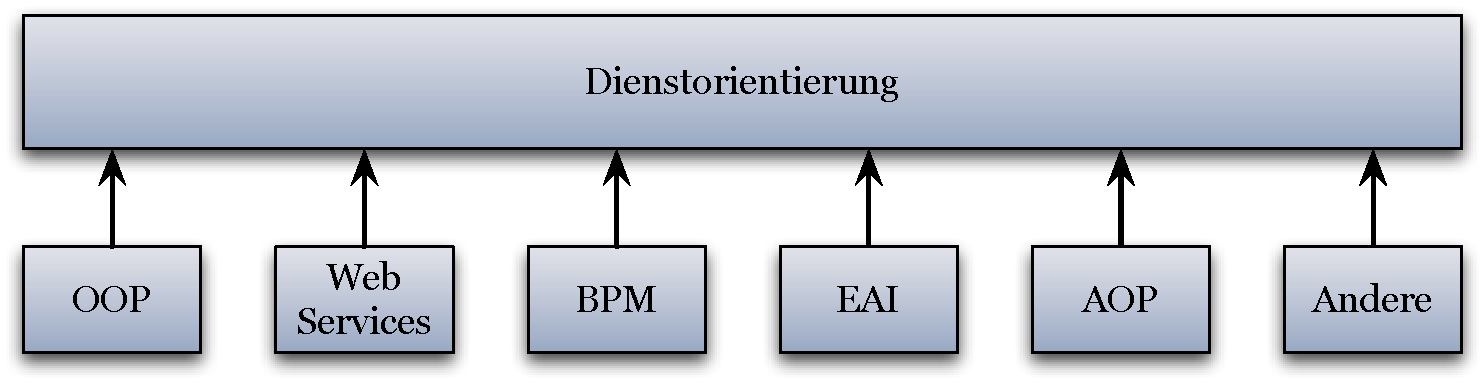
\includegraphics[width=.9\textwidth]{images/Wurzeln_Dienstorientierung.pdf}
  \caption{Einflüsse auf das Paradigma der Dienstorientierung nach~\citep{erl2008soa}}
  \label{fig:images_Wurzeln_Dienstorientierung}
\end{figure}

% subsubsection definition_dienstorientierung (end)

\subsubsection{Dienstorientierte Architektur} % (fold)
\label{ssub:definition_dienstorientierte_architektur}

  Bei der Definition von Natis wird zunächst die Schnittstelle zwischen den Diensten in den Vordergrund gerückt:

\begin{definition}[SOA (Natis)]\label{def:soa_natis_2003_}
  "`Essentially, SOA is a software architecture that starts with an interface definition and builds the entire application topology as a topology of interfaces, interface implementations and interface calls."'~\emph{\citep[S. 2]{natis2003soa}}
\end{definition}

  Obwohl die Konstruktion einer Architektur, die rund um definierte Schnittstellen aufgebaut wird, als Teilaspekt auch innerhalb einer SOA von Bedeutung ist, macht das allein noch keine dienstorientierte Architektur aus\footnote{Auch in der objektorientierten Programmierung gilt das Prinzip, dass gegen Interfaces und nicht gegen Implementierungen programmiert werden soll~\citep[S. 18]{design_patterns}.}. Die Definition der OASIS\abk{OASIS}{Organization for the Advancement of Structured Information Standards} fokussiert im Gegensatz dazu stärker auf den Aspekt der Verteiltheit und das einzelne Einheiten unterschiedlichen Domänen und Besitzern zugeordnet sein können:

\begin{definition}[SOA (OASIS Reference Model)]\label{def:soa_oasis_reference_model_}
  "`Service-Oriented Architecture (SOA) is a paradigm for organizing and utilizing distributed capabilities that may be under the control of different ownership domains."'~\emph{\citep[S. 8]{mackenzie2006rms}}
\end{definition}

  Nach Josuttis ist der Hintergrund der Softwareentwicklung die Abstraktion. Entscheiden ist lediglich nur aus welcher Perspektive die Abstraktion durchgeführt wird. Im Falle der dienstorientierten Architekturen findet diese Abstraktion aus Sicher der Geschäftsaspekte statt~\citep[S. 16]{soa_in_practice}. Darüber hinaus erweitert er die Definition der OASIS noch um die Größe der IT-Landschaft und stellt die Heterogenität der beteiligten Systeme heraus:

\begin{definition}[SOA (Josuttis)]\label{def:soa_josuttis_}
  "`SOA is an architectural paradigm for dealing with business processes distributed over a large landscape of existing and new heterogeneous systems that are under the control of different owners."'~\emph{\citep[S. 24]{soa_in_practice}}
\end{definition}

  Ein weiteres wesentliches Merkmal, vor allem auch für das COSIMA-Projekt, ist nach Papazoglou die technologische-agnostische Charakteristik der einzelnen Dienste. Zusätzlich beschreibt er die SOA als eine Meta-Architektur und betont die lose Kopplung der Dienste untereinander:

\begin{definition}[SOA (Papazoglou)]\label{def:soa_papazoglou_}
  "`[\ldots] SOA is a meta-architectural style that supports loosely coupled services to enable business flexibility in an interoperable, technology-agnostic manner."'~\emph{\citep[S. 257]{web_services_principles_and_technology}}
\end{definition}

  Papazoglou unterscheidet weiter zwischen zwei Arten dienstorientierter Architekturen, die sich jeweils im Grad ihrer Komplexität unterscheiden. Die einfachste Form einer SOA ist in Abbildung~\ref{fig:images_Basic_SOA} dargestellt.

  \begin{figure}[!ht]
    \centering
      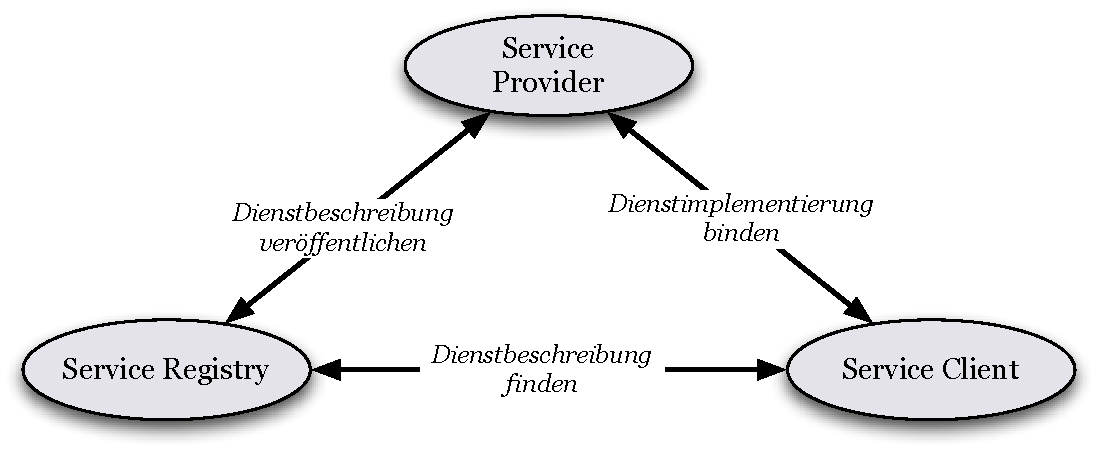
\includegraphics[width=.9\textwidth]{images/Basic_SOA.pdf}
    \caption{Einfachste Form einer dienstorientierten Architektur (nach~\citep{service_oriented_computing})}
    \label{fig:images_Basic_SOA}
  \end{figure}

  In diesem Modell sind zwar einige Eigenschaften einer SOA, wie sie in den vorangegangen Definitionen herausgestellt wurden, erfasst, jedoch bei weitem nicht alle. Lediglich die lose Kopplung und das sich Dienste auffinden lassen ist explizit modelliert. Alle anderen Eigenschaften, wie etwa Management, Dienstkomposition, Transaktionen zwischen und Koordination von Diensten oder Sicherheitsaspekte~\cite[S. 8]{service_oriented_computing} lassen sich wenn nur implizit wieder finden. Aus diesem Grunde stellt Papazoglou eine \emph{erweiterte} dienstorientierte Architektur (siehe Abbildung~\ref{fig:images_Extended_SOA}) vor, die diese Punkte explizit modelliert.

  \begin{figure}[!ht]
    \centering
      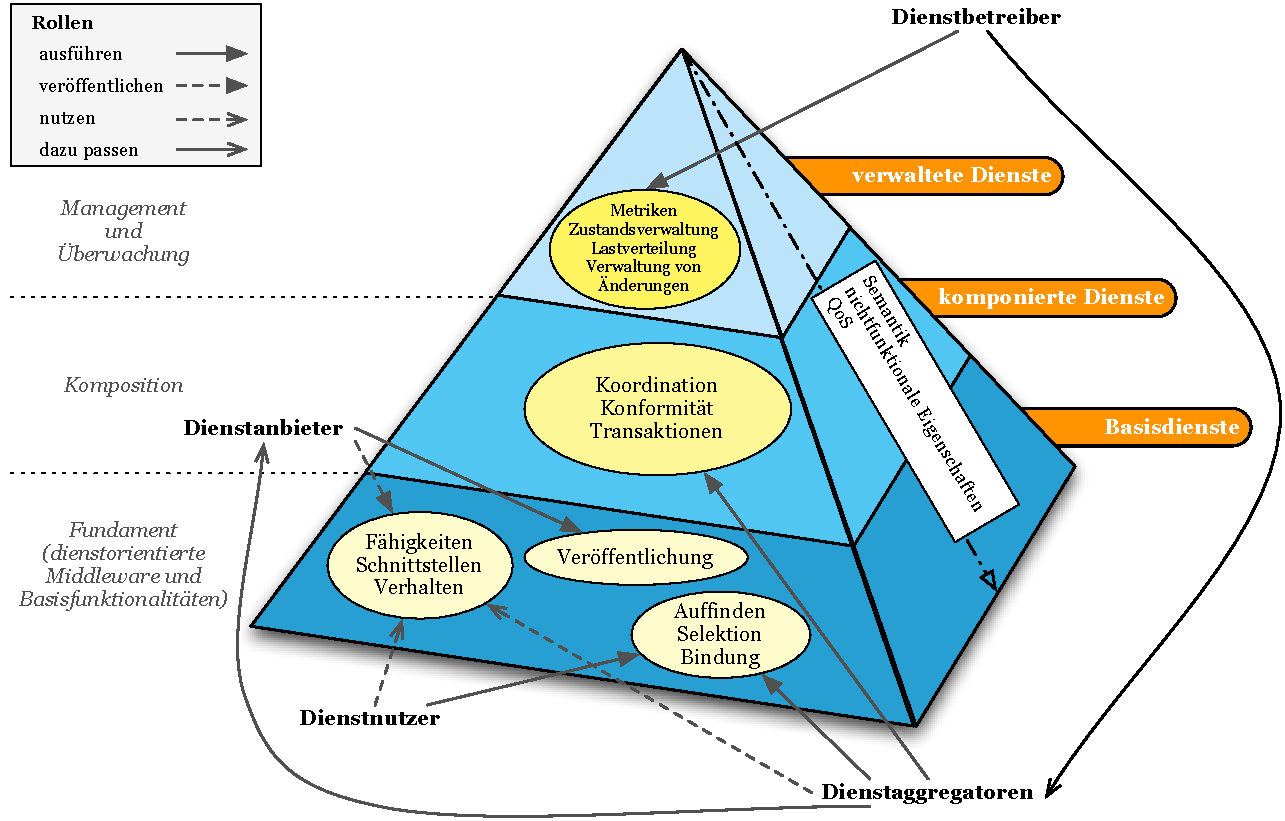
\includegraphics[width=.9\textwidth]{images/Extended_SOA.pdf}
    \caption{Erweiterte dienstorientierte Architektur nach Papazoglou~\citep{papazoglou2007soc}}
    \label{fig:images_Extended_SOA}
  \end{figure}

  Von besonderem Interesse im Kontext von COSIMA ist die Ebene der \emph{komponierten Dienste}. Auf dieser Ebene wird die Ausführung der einzelnen Dienste, sowie die Datenübertragung koordiniert~\cite[S. 8]{service_oriented_computing}. Auf dieser Ebene lassen sich müssen sich demnach die Mechanismen zur Synchronisation ($\to$ \ref{sub:synchronisation}) und Medienvermittlung ($\to$ \ref{ssub:media_broker}) befinden.
  
  In diesem, sehr viel umfangreicheren Modell, finden sich fast alle bisher vorgestellten Eigenschaften an eine SOA wieder. Vor allem der Aspekt, dass sich einzelne Dienste zu komplexeren Diensten zusammen fassen, also komponieren lassen, ist in diesem Modell prominent vertreten. Lediglich der Bezug zur (Geschäfts-)Prozessen ist nicht explizit modelliert. Die nachfolgende Liste fasst die wesentlichen Eigenschaften einer dienstorientierten Architektur noch einmal zusammen:

  \begin{itemize}
    \item Lose Kopplung
    \item Interoperabilität
    \item Dienste aus unterschiedlichen Domänen
    \item Bereitstellung einer Infrastruktur
    \item Architektur
    \item Komposition von Diensten zu Prozessen
    \item Betrachtung von nicht-funktionalen Anforderungen
  \end{itemize}

% subsubsection definition_dienstorientierte_architektur (end)

  Nach dieser Einordnung der wesentliche Begriffe, werden im Folgenden nun die einzelnen Komponenten der COSIMA Architektur im Detail vorgestellt.

% subsection definition_dienst_und_dienstorientierung (end)

\subsection{Einführung in COSIMA} % (fold)
\label{sub:einfuehrung}

  Bei der Konzeption und Entwicklung der Architektur sind unterschiedliche Sichten auf diese erstellt worden. Diese Sichten entsprechen denen von Starke in~\citep[S. 83]{effektive_software_architekturen} beschriebenen vier Arten von Sichten auf eine Software-Architektur: \emph{Kontextsichten}, \emph{Bausteinsichten}, \emph{Laufzeitsichten} und \emph{Verteilungssichten}.

  Für das COSIMA-Projekt wurden bisher Darstellungen aus zwei dieser Kategorien erstellt: eine der Kontextsichten und drei der Bausteinsichten. Die Kontextsichten legen laut Starke den "`Fokus auf den Zusammenhang oder das Umfeld des Systems"'~\citep[S. 87]{effektive_software_architekturen}, was auch auf die in Abbildung~\ref{fig:Kontextsicht_Architektur_COSIMA} dargestellte Kontextsicht von COSIMA zutrifft. Hier wird lediglich ein abstrakter und vor allem nicht formaler Überblick über die Architektur und beteiligte Systeme gegeben. Die Darstellungen, die sich den Bausteinsichten zuordnen lassen, sind namentlich das \emph{Komponentendiagramm}, das \emph{Kompositionsstrukturdiagramm} und der \emph{Grobentwurf} der Architektur. Diese finden sich jeweils in~\citep{bericht} und sollen an dieser Stelle nicht weiter betrachtet werden. Für die weitere Vorstellung der Architektur soll an dieser Stelle die Kontextsicht genügen.

  \begin{sidewaysfigure}[hp]
    \centering
    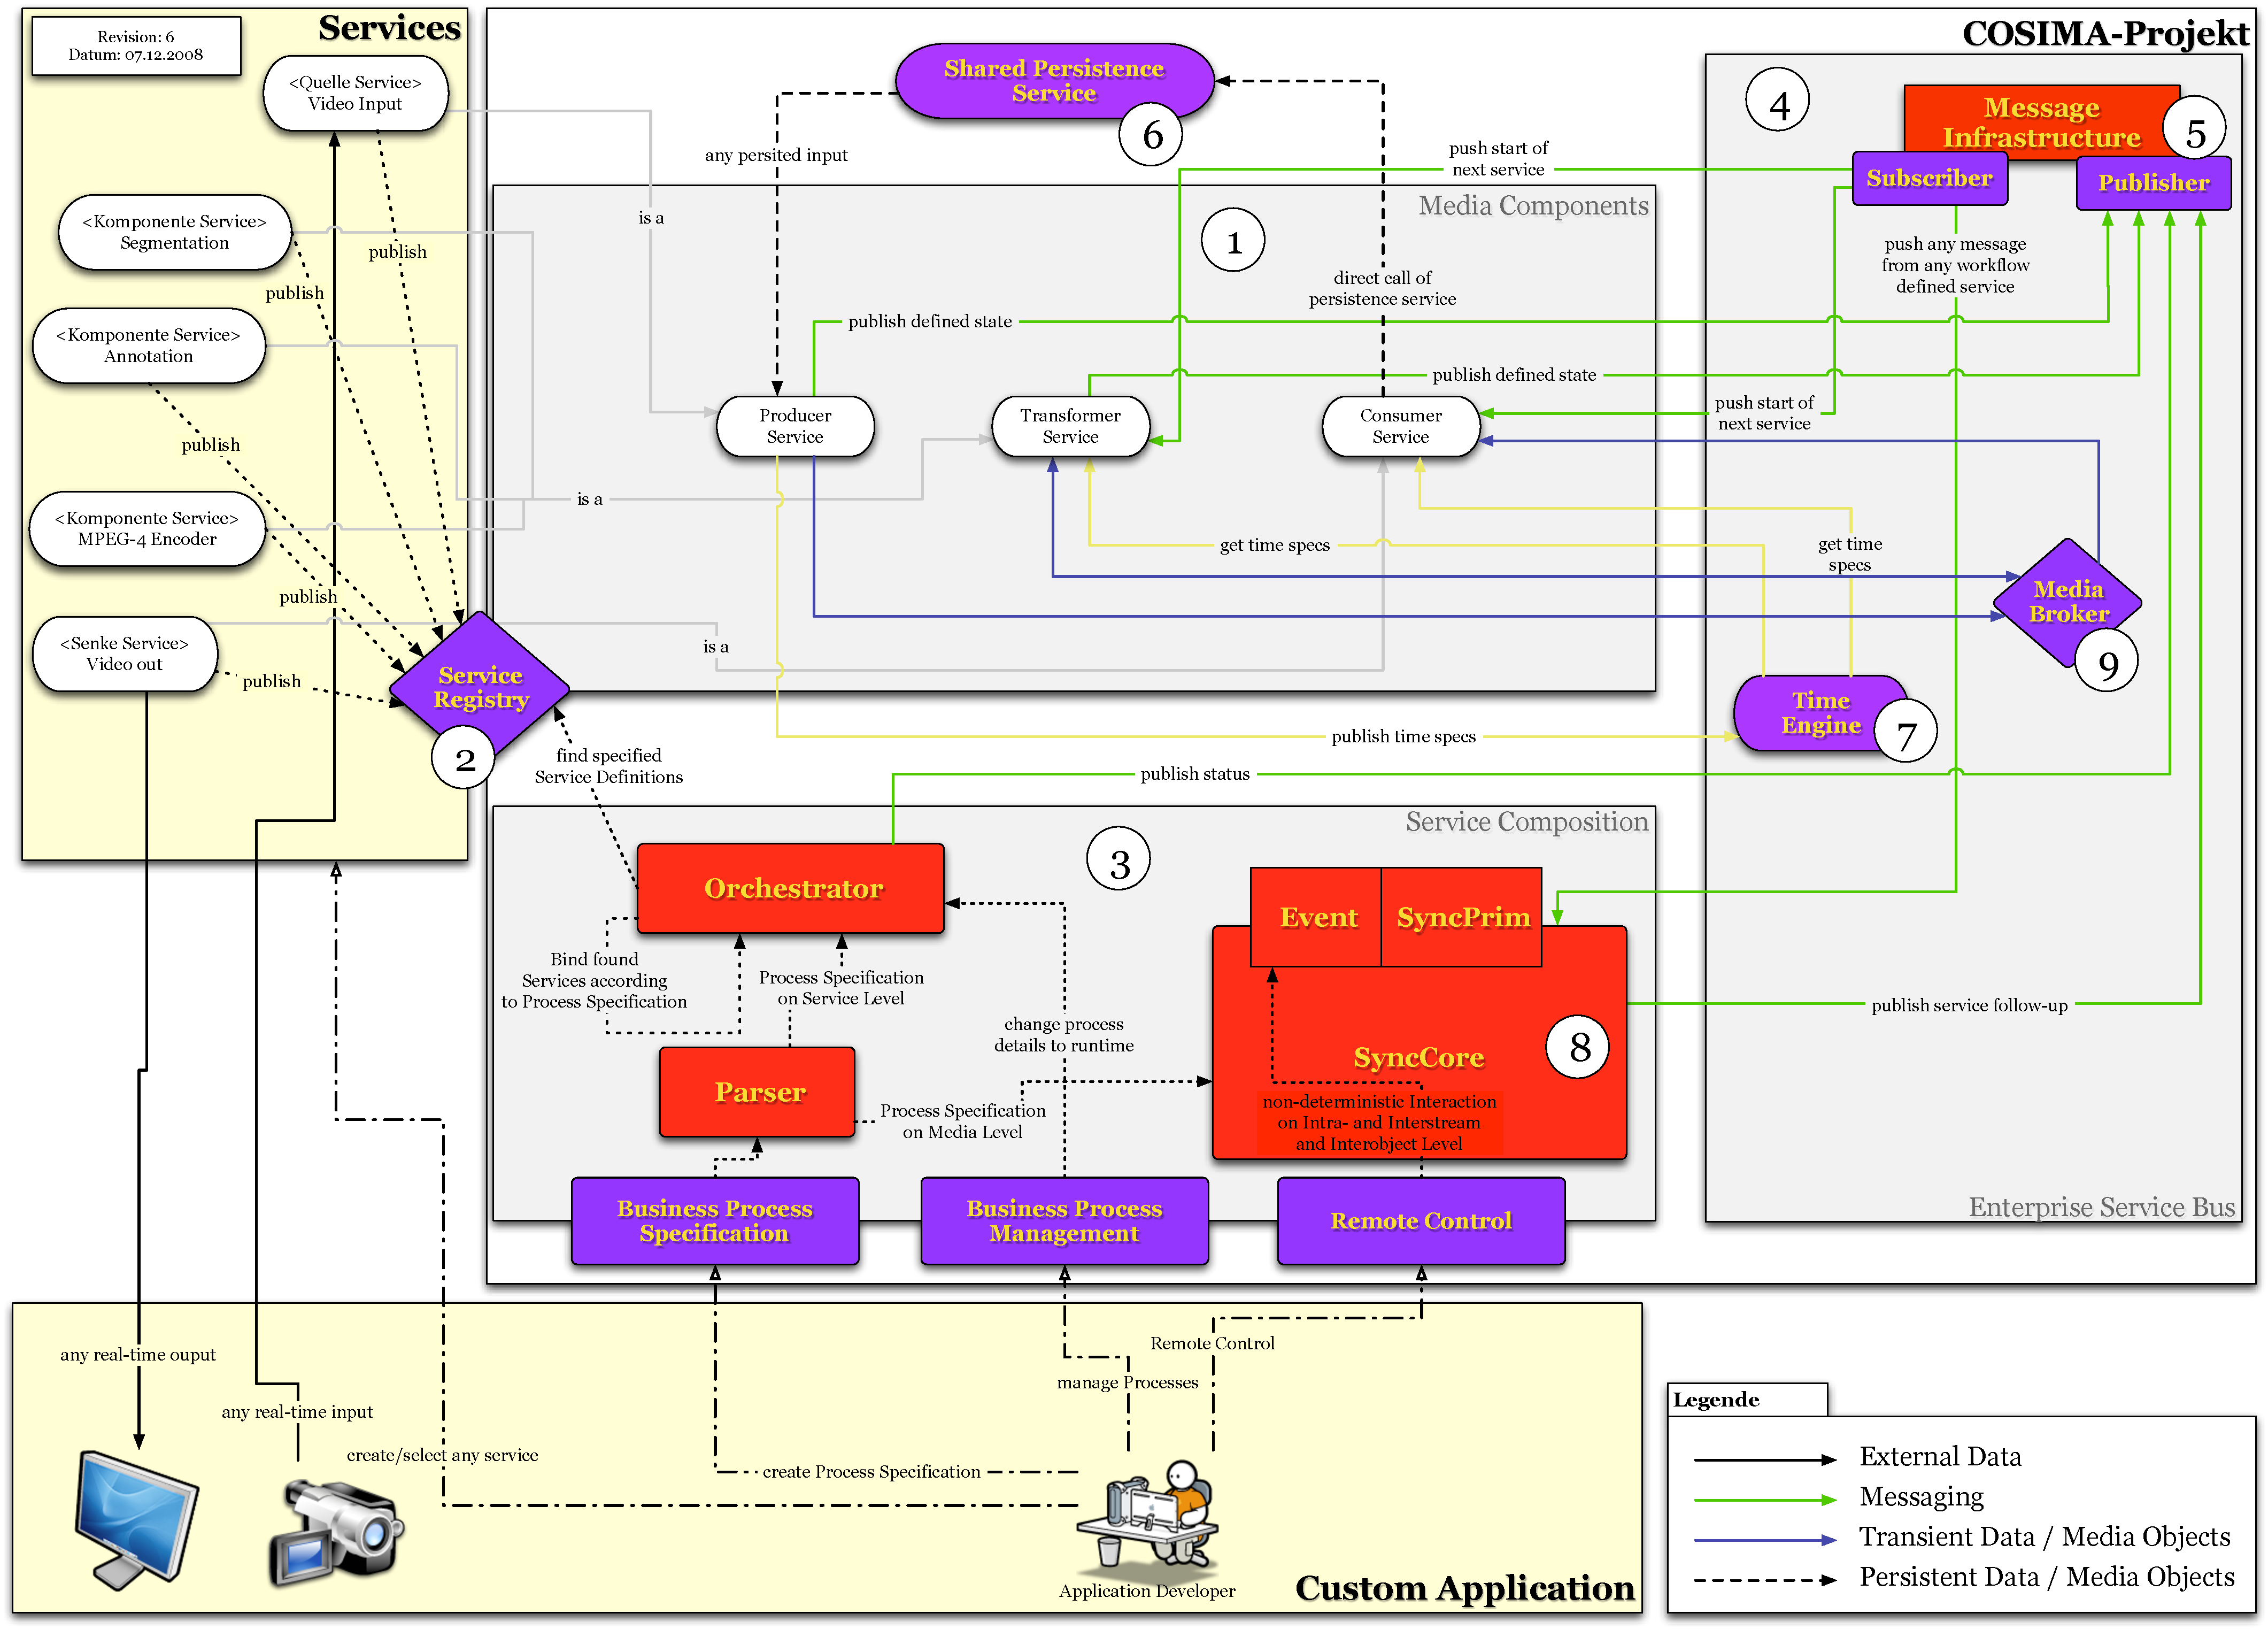
\includegraphics[width=\textwidth]{images/Kontextsicht_Architektur_COSIMA}
    \caption{Kontextsicht der Architektur des COSIMA-Projekts}
    \label{fig:Kontextsicht_Architektur_COSIMA}
  \end{sidewaysfigure}

  In der späteren prototypischen Realisierung und anschließenden Validierung der Architektur sollen und können nur Fragmente der Architektur umgesetzt werden, daher ist es sehr wichtig, solche Fragmente zu wählen, die für eine Weiterentwicklung von besonderem Interesse sind. Im Folgenden werden daher die zentralen Komponenten des COSIMA-Projekts kurz vorgestellt. \emph{Später soll dann eine Auswahl getroffen werden.}

  % - Kernpunkte der Architektur herausarbeiten
  % - Diese Kernpunkte müssen in der Realisierung/Validierung entsprechend besondere Berücksichtigung finden

% subsection einfuehrung (end)

\subsection{Medienverarbeitende Komponenten} % (fold)
\label{sub:medienverarbeitende_komponenten}

  Den Kern von COSIMA machen die medienverarbeitenden Komponenten aus, die vom Anwendungsentwickler in eine entsprechende Abfolge gebracht werden und damit die später Multimediaanwendung selbst darstellen: \emph{Producer}, \emph{Transformer} und \emph{Consumer}. Dem Entwurf der Komponenten liegt das \emph{Quelle-Komponente-Senke} Prinzip zu Grunde. Die innerhalb des COSIMA-Projekts verwendete Bezeichnung ist nach~\citep{a_multimedia_component_kit,multimedia_component_frameworks} ebenso valide wie die geläufigere Bezeichnung "`Quelle-Komponente-Senke"'. Da es sich bei COSIMA jedoch um eine komponentenbasierte Architektur handelt, kamen Benennungsschwierigkeiten auf, die die Verwendung einer alternativen Begrifflichkeit begünstigten.
  
  Diese medienverarbeitenden Komponenten sind dabei alle als Dienste, wie sie in der SOA verstanden werden, ausgeprägt. Zur Entwicklung einer Multimediaanwendung ist demnach eine Komposition dieser Dienste durch die in Abschnitt~\ref{sub:service_komposition} vorgestellten Ansätze notwendig. Eine formale Beschreibung der Dienste selbst wird im Service Registry vorgehalten, welches unter~\ref{sub:service_registry} näher erläutert wird.
  
  Der Austausch der zu verarbeitenden Medien zwischen den einzelnen Diensten geschieht auschließlich über den \emph{Media Broker}, der unter~\ref{sub:integration_von_medien} weiter ausgeführt wird. Ein genereller Nachrichtenaustausch zwischen den Diensten und mit den restlichen Teilen der Architektur wird über das Nachrichtensystem (\ref{ssub:nachrichtensystem}) realisiert. Persistenz von Daten und die Synchronisation werden von einem \emph{Persistence Data Service} bzw. der \emph{Timing Engine} übernommen. Beide Komponenten werden in~\ref{sub:infrastruktur} näher beschrieben. Teile dieser Architekturelemente sollen einmal in einem Service Bus aufgehen~\citep[S. 18]{bericht}.

% subsection medienverarbeitende_komponenten (end)

\subsection{Service Registry} % (fold)
\label{sub:service_registry}

  Wie bereits in Abschnitt~\ref{ssub:definition_dienstorientierte_architektur} gezeigt wurde, ist die Fähigkeit Dienste entdecken zu können eines der konstituierendes Element innerhalb einer SOA. Demnach ist auch in COSIMA eine solche vorgesehen. Nach~\citep{service_oriented_computing} ist diese selbst wieder als Dienst zu realisieren. Über die Registry lassen sich anhand von abstrakten (formalen) Dienstbeschreibungen konkrete Dienste identifizieren und eine Lokalisierung durchführen. Sie unterstützt damit die Forderung nach loser Kopplung innerhalb einer SOA. Eine Realisierung einer solchen Service Registry wäre beispielsweise durch UDDI\abk{UDDI}{Universal Description Discovery and Integration}\footnote{\url{http://www.oasis-open.org/committees/uddi-spec/}} oder ebXML\abk{ebXML}{Electronic Business using eXtensible Markup Language}\footnote{\url{http://www.ebxml.org/}} möglich.

% subsection service_registry (end)

\subsection{Servicekomposition} % (fold)
\label{sub:service_komposition}

  Als eine weitere wichtige Eigenschaft einer dienstorientierten Architektur ist die Fähigkeit zur Komposition von Diensten genannt worden. Ähnlich der Service Registry dient auch sie zur Entkopplung der einzelnen Dienste in einer SOA. Wesentlich entscheidender ist jedoch ihr Beitrag Dienste zu Prozessen zu aggregieren und damit neue Applikationen innerhalb einer dienstorientierten Architektur entwickeln zu können. Die Servicekomposition selbst setzt dabei auf die grundlegenden Elemente einer SOA auf~\citep[S. 51]{milanovic2004csw}, wie sie in Abschnitt~\ref{ssub:definition_dienstorientierte_architektur} vorgestellt wurden.
    
  Die Servicekomposition selbst kann dabei aus zwei unterschiedlichen Perspektiven betrachtet werden~\citep[S. 104]{masak2007ssb}: der \emph{Geschäftsprozesskomposition} und der \emph{Servicelevel-Komposition}. Bei der Geschäftsprozesskomposition werden "`völlig neue Geschäftsprozesse aus bestehenden Teilprozessen oder Services"' (\citep[S. 104]{masak2007ssb}) komponiert. Eine Einbettung in eine Organisation steht hier klar im Vordergrund. Bei der Servicelevelkomposition steht vielmehr "`die Interoperabilität und technische Machbarkeit im Vordergrund"' (\citep[S. 105]{masak2007ssb}) und es wird keine Rücksicht auf eine mögliche Organisationstruktur genommen.
  
\subsubsection{Kompositionsarten} % (fold)
\label{ssub:kompositionsarten}

  \textbf{BEDARF DIESER TEIL MEHR DISKUSSION!?}

  Bei der Komposition von Diensten werden in der Literatur verschiedene Vorgehen unterschieden. Die beiden grundsätzlichen, für COSIMA relevanten, werden bei Papazoglou in~\citep[S. 41]{papazoglou2007soc} genannt: \emph{Orchestrierung} und \emph{Choreographie}. Im Folgenden sollen diese beiden Ansätze genauer betrachtet werden.
  
\paragraph{Orchestrierung} % (fold)
\label{par:orchestrierung}
  
  Orchestrierung wird von Papazoglou wie folgt definiert:
  
  \begin{quote}
    \emph{"`Orchestration describes how services interact at the message level, including the business logic and execution order of interactions under control of a single end point. It is an executable business process that can result in a long-lived, transactional, multistep process model."'} (\citep[S. 41]{papazoglou2007soc})
  \end{quote}
  
  Wesentlich sind also die Interaktionen verschiedener Dienste, die von einer zentralen Stelle (dem \emph{single end point}) über einen Nachrichtenaustausch koordiniert und kontrolliert werden. Des Weiteren ist das Ergebnis ein ausführbarer Geschäftsprozess.

% paragraph orchestrierung (end)

\paragraph{Choreographie} % (fold)
\label{par:choreographie}

  In der Definition von~\citep{peltz2003wso} wird der Unterschied zwischen Choreographie und Orchestrierung deutlich:
  
  \begin{quote}
    \emph{"`[\ldots] choreography, which is more collaborative and allows each involved party to describe its part in the interaction. Choreography tracks the message sequences among multiple parties and sources -- typically the public message exchanges that occur between Web services -- rather than a specific business process that a single party executes."'} (\citep[S. 46]{peltz2003wso})
  \end{quote}

  Choreographie verfolgt also einen dezentralen Ansatz; Es gibt nicht eine Instanz, die den Nachrichtenfluss kontrolliert, vielmehr tritt der Nachrichtenfluss zwischen den einzelnen Diensten in den Vordergrund. Es liegt dadurch auch kein ausführbarer Prozess bei der Choreographie vor~\citep[S. 46]{peltz2003wso}.
  
  Für die konkrete Umsetzung dieser beiden Varianten zur Komposition existieren zahlreiche Technologien und Standards. Dabei fäll jedoch auf, dass eine strikte Trennung beider Ansätze auf der technischen Ebene eher künstlich erscheinen und daher in einem technologischen Ansatz vereint werden sollten~\citep[S. 42]{papazoglou2007soc}.
  
  Eine detaillierte Auseinandersetzung mit der Thematik der Geschäftsprozesskomposition und -modellierung im Rahmen des COSIMA-Projekts findet sich in der Master Thesis von Matthias Richter~\citep{samma08}.

% paragraph choreographie (end)

% subsubsection kompositionsarten (end)

% \subsubsection{Relevanz fuer COSIMA} % (fold)
% \label{ssub:relevanz_fuer_cosima_komposition}
% 
%   Es wurde deutlich, dass die Servicekomposition für eine dienstorientierte Architektur von elementarer Bedeutung ist. Jedoch wurde auch klar, dass die Servicekomposition in COSIMA noch nicht so verstanden wird, wie sie in der Literatur verstanden wird; Dort findet eine Betrachtung im Kontext von Geschäftsprozessen statt. Sowohl in der bisherigen Zieldefinition von COSIMA, als auch in dem Szenario für die prototypische Realisierung der Architektur, dass in Kapitel~\ref{cha:szenario} vorgestellt wird, liegt der Fokus jedoch nicht auf Geschäftsprozessen. Daher ist auch eine weitere Betrachtung der genannten Details für diese Arbeit nicht notwendig. Dennoch kann festgehalten werden, dass es sich am ehesten um eine Orchestrierung handelt: Es existiert eine zentrale Komponente über die der Anwendungsentwickler die Möglichkeit erhält, die unterschiedlichen Funktionalitäten der Multimedia-Applikationen zu komponieren und in eine definierte Abfolge zu bringen.

% subsubsection relevanz_fuer_cosima (end)

  % - Definitionen von "`Workflow"' und "`Prozess"' in Zusammenhang auf die Entwürfe (vielleicht )
  % - BPEL/Orchestrierung/Choreographie mit Quellenangaben erläutern
  % - vielleicht macht dieser Abschnitt überhaupt keinen Sinn!
  % - Die grundsätzliche Möglichkeit der Verwendung einer Prozessbeschreibungssprache diskutieren
  
% subsection service_komposition (end)

\subsection{Infrastruktur und ESB} % (fold)
\label{sub:infrastruktur}

  Innerhalb einer dienstorientierten Architektur besteht der Bedarf nach einer Infrastruktur, die in der Lage ist, die einzelnen Dienste zu verwalten und zu integrieren~\citep[S. 270]{web_services_principles_and_technology}. Neben der bereits separat vorgestellten Servicekomposition gehören auch die in diesem Abschnitt vorgestellten Elemente dieser, in der Literatur als \emph{Enterprise Service Bus} (ESB\abk{ESB}{Enterprise Service Bus}) bezeichneten Infrastruktur an.
  
  In~\citep{web_services_principles_and_technology} wird der Enterprise Service Bus wie folgt defniert:
  
  \begin{definition}[ESB]\label{def:enterprise_serivce_bus}
    "`The Enterprise Service Bus is an open standards-based message backbone designed to enable the implementation, deployment, and management of SOA-based solutions with a focus on assembling, deploying, and managing distributed service-oriented architectures."'~\emph{\citep[S. 270]{web_services_principles_and_technology}}
  \end{definition}
  
  Nach dieser Definition wird durch den Einsatz eines ESB überhaupt erst die Realisierung und der Betrieb einer dienstorientierten Architektur ermöglicht. Darüber hinaus lässt sich festhalten, dass auch das "`Assembling"' der einzelnen Teile innerhalb der Architektur in den Aufgabenbereich des ESB fallen. Demnach kann die Servicekomposition in einer SOA auch als eine Teilmenge des ESB angesehen werden~\citep[S. 3]{enterprise_service_bus}.

  Neben der Servicekomposition werden von dem ESB noch eine Vielzahl weiterer Aufgaben übernommen, die jeweils die Punkte Implementierung, Deployment\footnote{Das englische Wort "`Deployment"' kann in diesem Kontext am ehesten mit "`Inbetriebsetzung"' übersetzt werden. Da sich "`Deployment"' jedoch in der Fachsprache weitestgehend eingeprägt hat, wird es sinngemäß nach der Beschreibung in der Wikipedia verwendet: \emph{"`Software deployment is all of the activities that make a software system available for use."'} (aus Wikipedia: \url{http://en.wikipedia.org/wiki/Software_deployment}, zuletzt abgerufen am 22.10.2008)} und Management unterstützen sollen. Die Aufgaben, die im ESB dabei mindestens implementiert sein müssen, sind in der folgenden Liste nach~\citep[S. 137]{soa_goes_real} und~\citep[S. 146]{masak2007ssb} dargestellt:
  
  \begin{itemize}
    \item Routing von Nachrichten
    \item Kommunikationsbus als Integrationsgrundlage
    \item Datentransformation und -zuordnung
    \item Prozess- und Regelausführung
    \item Überwachung der einzelnen Komponenten
    \item Adaptoren für Applikationen
    \item Bereitstellen von standardisierten Schnittstellen
  \end{itemize}

  Historisch gesehen ist ein ESB die Weiterentwicklung von EAI Brokern\abk{EAI}{Enterprise Application Integration}, die bereits ähnliche oder gleiche Funktionalitäten bereitstellen konnten~\citep[S. 146]{masak2007ssb}. Der Enterprise Service Bus verzichtet dabei aber auf den zentralistischen Integrationsansatz von EAI Brokern und etabliert anseinerstatt eine verteilte Integration~\citep[S. 4]{enterprise_service_bus}. Die einzelnen Funktionalitäten werden, um diese Verteiltheit zu erreichen, selbst wieder als Dienste realisiert ~\citep{enterprise_service_bus,masak2007ssb,papazoglou2007soc}. Durch die Aufteilung in einzelne Dienste und deren Verteilung innerhalb des Service Bus, kann dann auch von einer virtuellen Infrastruktur gesprochen werden~\citep[S. 136]{soa_goes_real}.
  
  Das COSIMA Projekt sieht bis zu diesem Zeitpunkt nur einen sehr rudimentären ESB vor\footnote{Gemessen an dem Umfang, wie er in der Literatur beschrieben wird und in kommerziellen Systemen vorkommt.}. Dennoch übernimmt auch der Enterprise Service Bus in COSIMA die gleichen Verantwortlichkeiten, einige davon sind jedoch für den Einsatz in Multimediaanwendungen adaptiert worden. Im Folgenden werden die für das COSIMA Projekt relevanten Komponenten des ESBs näher beschrieben.
  
\subsubsection{Nachrichtensystem} % (fold)
\label{ssub:nachrichtensystem}
  
  Im vorangegangen Kapitel wurde als eine Aufgabe des Enterprise Service Bus, die Vermittlung und Übertragung von Nachrichten zwischen den einzelnen Teilnehmern genannt. Das \emph{Messaging}, also die Nachrichtenvermittlung ist immer das Herzstück eines ESB~\citep[S. 77]{enterprise_service_bus} und daher auch in COSIMA. Die Nachrichtenvermittlung dient dabei dazu eine sehr schnelle, asynchrone und verlässliche Kommunikation zwischen Applikationen zu realisieren. Eine Nachricht selbst ist dabei ein wohl-definiertes, datengetriebenes Textformat~\citep[S. 60f]{web_services_principles_and_technology}.
  
  In COSIMA wurde sich für ein Nachrichtensystem nach dem \emph{Publish/Subscribe}-Pattern entschieden~\citep[S. 106]{enterprise_integration_patterns}. Es ist eine von vielen Formen, um asynchrone und verlässliche Kommunikation zu realisieren, die dabei etwas besser skaliert als andere Lösungen~\citep[S. 69]{web_services_principles_and_technology}. Zusammengefasst lässt sich die Funktionsweise dieser Form der Nachrichtenvermittlung wie folgt beschreiben:
  
  \begin{itemize}
    \item Ein \emph{Publisher} veröffentlicht eine Nachricht zu einem bestimmten Thema.
    \item Alle \emph{Subscriber}, die dieses Thema abonniert haben, erhalten genau eine Kopie dieser Nachricht.
  \end{itemize}
  
  Bei~\citep[S. 127]{soa_goes_real} wird darüber hinaus gesagt, dass es sich bei dieser Form der Nachrichtenvermittlung, um eine nicht-gerichtete Kommunikation handelt.
  
  In COSIMA selbst werden über das Nachrichtensystem vor allem Kontroll- und Synchronisationsdaten vermittelt. Die Kontrolldaten werden dabei von der Komponente der Servicekomposition versendet, und beinhalten Informationen wo und wie die medienverarbeitenden Komponenten ihre Daten beziehen können. Das Nachrichtensystem soll nämlich nicht die Medien selbst vermitteln. Für diese Aufgabe wurde eine dedizierte Komponente eingeführt, die in Abschnitt~\ref{sub:integration_von_medien} näher beschrieben wird. Auf die Synchronisationsdaten wird in Abschnitt~\ref{ssub:synchronisation} näher eingegangen.
  
% subsubsection nachrichtensystem (end)

\subsubsection{Persistenz} % (fold)
\label{ssub:persistenz}

  Um Daten zu dauerhaft ablegen zu können, ist innerhalb von COSIMA ein weiterer Dienst vorgesehen worden, der \emph{Shared Persistence Service}. Allerdings kann nur eine \emph{Consumer}-Komponente über diesen Dienst ablegen lassen. Umgekehrt kann nur eine \emph{Producer}-Komponente Daten über diesen Dienst wieder einlesen. Eine \emph{Transformer}-Komponente, kann nach dem Quelle-Komponente-Senke Prinzip keinen Zugriff auf dauerhaft abgelegte Daten erhalten.
  
  Innerhalb von COSIMA ist dieser Dienst noch sehr rudimentär modelliert. In der Literatur zu SOA findet sich keine dedizierte Komponente, um Daten persistent zu speichern; Diese Funktionalität kann durch jeden beliebigen Dienst bereitgestellt werden. Auf Grund dieser Tatsache und durch die Etablierung eines dedizierten Medien Brokers ($\to$ \ref{ssub:medienobjekt}), der die Vermittlung der Medienobjekte realisiert, ist die weitere Existenzberechtigung dieser Komponente jedoch eher zweifelhaft. Eine weitere Betrachtung dieser Zusammenhänge findet in Abschnitt \ref{sub:integration_von_medien} statt.
  
% subsubsection persistenz (end)

  Die bis hierher vorgestellten Komponenten der Architektur innerhalb des COSIMA-Projekts sind weitestgehend übertragbar auf Komponenten in anderen dienstorientierten Architekturen. Zur Umsetzung von Multimediaanwendungen sind aber noch weitere, medienspezifische Komponenten erforderlich. Auch wenn sie sich grundsätzlich dem Enterprise Service Bus zuordnen lassen, sollen sie dennoch dediziert im nächsten Abschnitt diskutiert werden.

% subsection infrastruktur (end)

\subsection{Integration von Medien} % (fold)
\label{sub:integration_von_medien}

  Die in diesem Abschnitt vorgestellten Komponenten tragen maßgeblich dazu bei, dass sich mit COSIMA Multimediaanwendungen realisieren lassen. Um jedoch die Relevanz dieser Komponenten im Rahmen von Multimedia begreifen zu können, soll im ersten Schritt eine Definition des Begriffs Multimedia gegeben werden, aus dem sich dann später die Anforderungen an die hier vorgestellten Komponenten ableiten lassen.
  
\subsubsection{Definition: Multimedia} % (fold)
\label{ssub:definition_multimedia}
  
  Verbaliter lässt sich Multimedia durch die Bedeutung der beiden Wortteile "`Multi-"' und "`Media"' oder "`Medium"' erschließen:

  \begin{definition}[Multi-]\label{def:multi_}
    "`vielfach, mehrer\ldots, viel\ldots/Viel\ldots"'\footnote{aus: Duden - Deutsches Universal Wörterbuch A-Z, 3. Aufl., 1996}
  \end{definition}
  
  \begin{definition}[Medium / Medien]\label{def:medium}
    "`\textbf{Medium} (lat. »Mitte«) \textbf{1.} bildungssprachlich für: vermittelndes Element [\ldots] \textbf{3.} Kommunikationswissenschaften: Vermittlungsinstanz von Informationen [\ldots]. \textbf{Medien} (von engl. »media«), Sg. Medium, Sammel-Bez, für alle techn. Mittel zur Verarbeitung von Information, d.h. für Kommunikationsmittel (z.B. Zeitung, Zeitschrift, Buch, Plakat, Hörfunk, Fernsehen, Internet) [\ldots]"'\footnote{aus: Brockhaus - die Enzyklopädie, 21. Auflage, 2006}
  \end{definition}
  
  Der Begriff \emph{Multimedia} ließe sich daher so definieren, dass es sich um viele vermittelnden Instanzen von Informationen handelt. Diese Definition wäre für den konkreten Kontext jedoch zu unspezifisch und es ist daher eine weitere Einordnung notwendig.
  
  Bei Steinmetz wird die genannte Definition dahingehend erweitert, dass ein Medium "`ein Mittel zur Verbreitung und Darstellung von Informationen"'~\citep[S. 7]{multimedia_technologie} ist. Sie wird also explizit um die \emph{Darstellung} von Informationen ergänzt. Noch weiter lässt sich der Begriff \emph{Medium} nach den folgenden Kriterien differenzieren: Perzeptions-, Repräsentations-, Präsentations-, Speicher-, Übertragungs-, und Informationsaustauschmedien. Dabei entsprechen die Perzeptionsmedien am nächsten dem, was in einer Multimediaanwendungen under Medien verstanden wird: Die Informationen, die der Mensch mit seinen fünf Sinnen wahrnehmen kann~\citep[S. 9]{multimedia_technologie}\footnote{Dies bedeutet im Umkehrschluss jedoch nicht, dass die anderen Arten von Medien keine Rolle spielen.}. Jedes Medium definiert dabei einen \emph{Darstellungsraum} mit entsprechenden \emph{Darstellungsdimensionen}. Neben dem räumlichen Dimensionen dient vor allem die zeitlich Dimension dazu, eine weitere Einordnung von Medien vornehmen zu können~\citep[S. 10]{multimedia_technologie}:
  
  \begin{description}
    \item[Diskrete Medien] Medien, deren Informationen zeitunabhängig auftreten, etwa Text oder Grafik. Ihre Verarbeitung ist zeitunkritisch.
    \item[Kontinuierliche Medien] Medien, deren Informationen sich über die Zeit hinweg ändern, etwa Ton oder Video. Ihre Verarbeitung ist zeitkritisch.
  \end{description}

  Mit dieser Erkenntnis wäre es nicht angemessen, den Begriff Multimedia rein quantitativ zu beschreiben, sondern viel mehr ist eine qualitative Definition adäquat:

  \begin{definition}[Multimedia]\label{def:multimedia}
    "`Als Multimedia wird der Einsatz von sowohl mindestens einem diskreten und mindestens einem kontinuierlichem Medium verstanden."'~\emph{\citep[S. 14]{multimedia_technologie}}
  \end{definition}
  
  Aufbauend auf dieser Definition von Multimedia kann abschließend auch der Begriff \emph{Multimediaanwendungen} oder \emph{Multimediasystem} definiert werden:

  \begin{definition}[Multimediasystem]\label{def:multimediasystem}
    "`Ein Multimediasystem ist durch die rechnergesteuerte, integrierte Erzeugung, Manipulation, Darstellung, Speicherung und Kommunikation von unabhängigen Informationen gekennzeichnet, die in mindestens einem kontinuierlichen (zeitabhängigen) und einem diskreten (zeitunabhängigen) Medium kodiert sind."'~\emph{\citep[S. 13]{multimedia_technologie}}
  \end{definition}
  
% subsubsection definition_multimedia (end) 

  Obwohl die Informationen selbst unabhängig voneinander sind, so muss in der Regel dennoch ein Bezug zwischen den einzelnen Informationen hergestellt werden können. Dieser Bezug wird auch \emph{Synchronisation} genannt und im nächsten Abschnitt näher beschrieben.

\subsubsection{Synchronisation} % (fold)
\label{ssub:synchronisation}

  An sich unabhängige Medien müssen in der Regel in einer Multimediaanwendungen in einen Zusammenhang gebracht werden; Beispielsweise muss ein Video in einen Zusammenhang mit Untertiteln gebracht werden. Die Etablierung dieses Zusammenhangs wird als \emph{Synchronisation} bezeichnet. Allgemein kann sie als das "`Herstellen des Gleichlaufs von Vorgängen, Maschinen u. a."'\footnote{aus: Der Brockhaus in einem Band. 10. Auflage, 2005} bezeichnet werden. Wie bereits bei der allgemeinen Definition von Multimedia, ist auch diese zu unspezifisch für den gegebenen Einsatz und auch hier muss eine weitere Klassifikation stattfinden. Bereits aus dem Eingangs genannten Beispiel lassen sich separate Eigenschaften extrahieren: Nicht nur müssen die Untertitel zur rechten Zeit angezeigt werden, sondern sie haben auch im Videobild selbst eine räumliche Positionierung. Es existiert also eine \emph{zeitliche} wie \emph{örtliche} Beziehung statt. Neben diesen beiden Arten von Beziehungen existiert noch eine Weitere, die \emph{Inhaltliche}:
  
  \begin{description}
    \item[Inhaltliche Beziehung] Definiert die Abhängigkeit einzelner Medien von bestimmten Daten.
    \item[Örtliche Beziehung] Ist auch bekannt als \emph{Layout} Beziehung und definiert die Beziehung von unterschiedlichen Medien im Raum, bezogen auf ein Ausgabegerät zu einem bestimmten Zeitpunkt.
    \item[Zeitliche Beziehung] Definiert die zeitlichen Abhängigkeiten von Medien und ist immer dann von Bedeutung, wenn mit kontinuierlichen Medien umgegangen wird.
  \end{description}
  
  Alle drei Arten müssen in einer Multimediaanwendungen betrachtet werden und müssen daher auch im COSIMA-Projekt berücksichtigt werden. Synchronisation wird eigentlichen Sinne jedoch auf die zeitliche Beziehung von unterschiedlichen Medien~\citep[S. 572]{steinmetz1995mcc} angewandt. Diese besondere Bedeutung der zeitlichen Komponente bei der Betrachtung von Multimediadaten wurde auch von Bertino und Ferrari festgestellt:

  \begin{quote}
    \emph{"`One of the inherent characteristics of multimedia data is of being heavily time-dependent in that they are usually related by temporal relations which have to be maintained during their playout."'} (\citep[S. 612]{bertino1998tsm})
  \end{quote}
  
   Auf Grund der besonderen Relevanz der Zeitdomäne soll im Rahmen dieser Arbeit die folgende Definition von Synchronisation Geltung besitzen: 
  
  \begin{definition}[Synchronisation]\label{def:synchronisation}
    "`Synchronization in the context of multimedia refers to the mechanisms used by processes (also specific to multimedia) to coordinate their ordering in the time domain."'~\emph{\citep[S. 401]{steinmetz1990spm}}
  \end{definition}
  
  Nach dem eine Definition für Synchronisation gefunden wurde, sollen im weiteren Verlauf unterschiedliche Ansätze zur Modellierung von zeitlicher Synchronisation in Multimediaanwendungen vorgestellt werden.
  
\minisec{Modelle zur Beschreibung zeitlicher Synchronisation} % (fold)
\label{msec:modelle_zur_beschreibung_zeitlicher_synchronisation}

  Um zeitliche Synchronisation zu beschreiben und in einer Multimediaanwendungen abbilden zu können, existieren unterschiedliche Modelle und Klassifikationen, von denen eine für diesen Kontext relevante Auswahl hier näher beschrieben werden soll.
  
\paragraph{Natürliche und Synthetische Synchronisation} % (fold)
\label{par:natuerliche_und_synthetische_synchronisation}

  Eine erste Klassifikation kann über eine Unterscheidung in \emph{natürliche} (oder \emph{live}) und \emph{synthetische} Synchronisation~\citep{little1991ms,little1991msp,steinmetz1992mst} erstellt werden. Bei der natürlichen Synchronisation wird die zeitliche Beziehung zwischen den einzelnen Medien implizit während der Aufnahme erfasst. In der Regel tritt eine natürliche Synchronisation nur bei kontinuierlichen Medien auf. Im Gegensatz dazu definiert die synthetische Synchronisation die zeitlichen Beziehung explizit über eine Spezifikation. Bei der natürlichen Synchronisation besteht das Ziel darin, dass die zeitlichen Beziehung, die während der Aufnahme der Medien implizit mit erfasst wurden, bei der Präsentation immer noch Geltung besitzen. Die synthetische Synchronisation wird die Möglichkeit gegeben möglichst flexibel zeitliche Abhängigkeiten zu modellieren, die dann auch wieder bei der Präsentation Geltung haben müssen~\citep[S. 613]{bertino1998tsm}. Im COSIMA-Projekt müssen in jedem Fall beide Variante Berücksichtigung finden.
  
% paragraph nat_rliche_und_synthetische_synchronisation (end)

\paragraph{Granularität von Synchronisation} % (fold)
\label{par:granularitaet_von_synchronisation}

  Neben der Klassifikation, ob eine Synchronisation implizit oder explizit erfasst wurde, lassen sich ebenfalls unterschiedliche Granularitäten von zeitlichen Beziehungen unterscheiden, die in Abbildung \ref{fig:granularitaetsebenen} exemplarisch dargestellt und im Anschluss beschrieben sind.
  
  \begin{figure}[!ht]
    \centering
      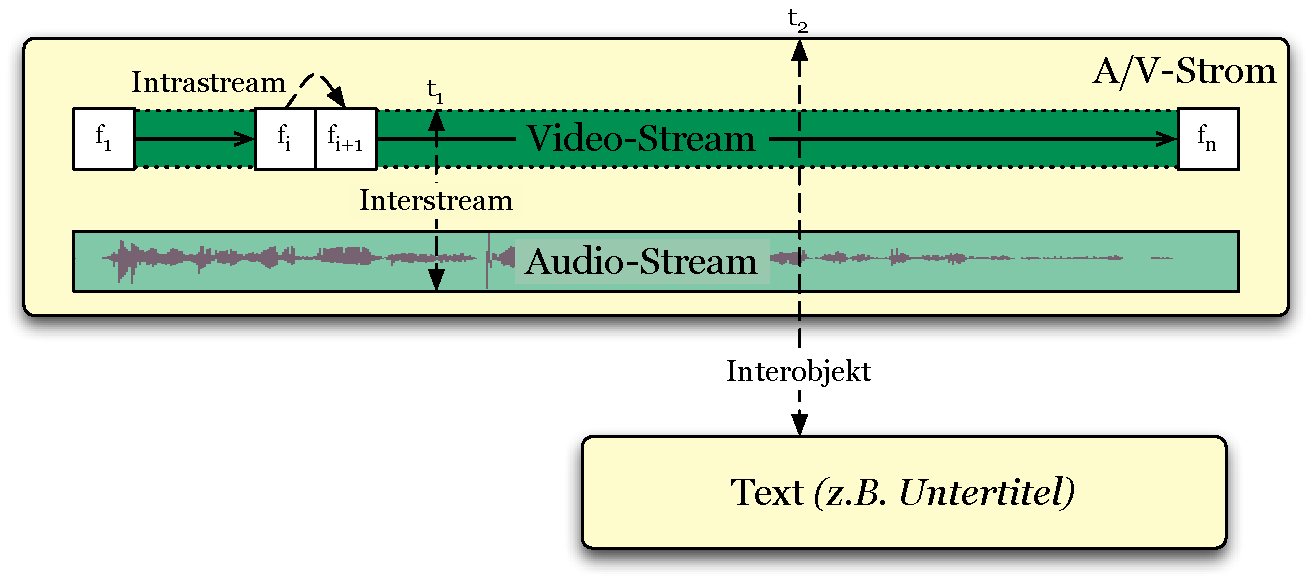
\includegraphics[width=.9\textwidth]{images/Granularitaetsebenen.pdf}
    \caption{Die drei Granularitätsebenen auf denen Synchronisation stattfinden kann (nach~\citep{antons09})}
    \label{fig:granularitaetsebenen}
  \end{figure}
  
  \begin{description}
    \item[Intrastream] Die Intrastream-Synchronisation bezieht auf die einzelnen \mbox{(Präsentations-)} Einheiten innerhalb eines Objekts. Diese Einheiten werden auch als Logische Dateneinheiten (\emph{Logical Data Units} (LDU\abk{LDU}{Logical Data Units})) bezeichnet~\citep{steinmetz1990spm}.
    \item[Interstream] Die Interstream-Synchronisation bezieht sich auf verschiedene Ströme innerhalb einer Stromgruppe~\citep{multimedia_technologie}, etwa die zeitliche Beziehung von einer Ton- und Videospur in einem A/V-Strom\footnote{Im MET++-Rahmenwerk werden für Intrastream und Interstream die Begriffe \emph{Intramedia (low-level)} und \emph{Intermedia (high-level)} verwendet~\citep[S. 73]{ackermann1996doo}.}.
    \item[Interobjekt] Im Zusammenhang mit der Referenzarchitektur nach Meyer und Steinmetz ($\to$ \ref{par:referenzmodelle}) ist es in Betracht zu ziehen, diese zusätzliche Granularitätsebene einzuführen~\citep[S. 264]{wu2001svo}, die zwischen verschiedenen Medienobjekten zeitliche Beziehungen herstellt. In der Literatur lässt sich dazu jedoch keine einheitliche Aussage finden, aber auch in Bezug auf eine verteilte Architektur kann diese Unterscheidung von Vorteil sein. Eine abschließende Betrachtung kann im Rahmen dieser Arbeit jedoch nicht erfolgen.
  \end{description}
  
  Im Folgenden Abschnitt werden diese Ebenen in ein Referenzmodell zur Multimedia-Synchronisation eingeordnet.

% paragraph granularität_von_synchronisation (end)

\paragraph{Referenzmodelle} % (fold)
\label{par:referenzmodelle}

  Um ein besseres Verständnis über die Anforderungen an eine Multimedia-Synchronisation bilden zu können und verschiedene Multimedia-Synchronisationsysteme miteinander zu vergleichen, ist ein Referenzmodell notwendig~\citep[S. 601]{multimedia_technologie}. In der Fachliteratur existieren eine Reihe von potentiell geeigneten Modellen~\citep[S. 601]{multimedia_technologie}. Eines davon ist das Referenzmodell nach Little und Ghafoor~\citep{little1991ms}. Es unterscheidet zwischen einer \emph{physikalischen Ebene}, \emph{Systemebene} und einer \emph{menschlichen Ebene}, lässt dabei aber eine detaillierte Beschreibung von Klassifikationskriterien vermissen~\citep[S. 601]{multimedia_technologie}. Auch andere Modelle verfolgen nach Steinmetz einen eher orthogonalen Ansatz~\citep[S. 601]{multimedia_technologie}. Wesentlich besser, auch für die Zwecke von COSIMA lässt sich das Referenzmodell nach Meyer et al.~\citep{meyer1993tms} verwenden, dass in seiner durch Steinmetz weiterentwickelt Form~\citep{steinmetz1995mcc} in Abbildung \ref{fig:images_Erweiterte_Synchronisations-Ebenen} dargestellt ist. Zu seinem Vorgänger unterscheidet es sich dabei vor allem in der zusätzlichen Spezifikationsschicht\footnote{In diesem Referenzmodell bietet jede höhere Ebene neben einer stärkeren Abstraktion in der Programmierung zusätzlich auch eine stärkere Abstraktion bei der Behandlung der \emph{Dienstgüte} (\emph{Quality of Service} (QoS\abk{QoS}{Quality of Service}))~\citep[S. 601]{steinmetz1995mcc}.}.

  \begin{figure}[!ht]
    \centering
      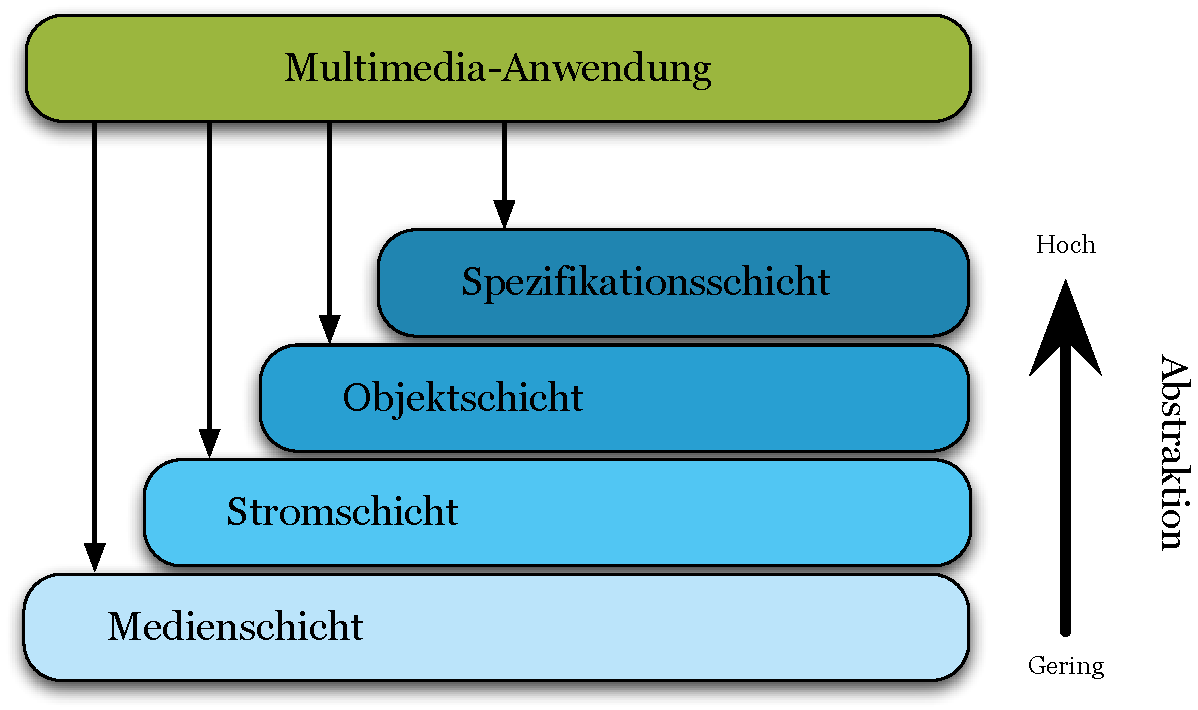
\includegraphics[width=.9\textwidth]{images/Erweiterte_Synchronisations-Ebenen.pdf}
    \caption{Erweiterte Ebenen der Synchronisation, nach~\citep[S. 601]{steinmetz1995mcc}}
    \label{fig:images_Erweiterte_Synchronisations-Ebenen}
  \end{figure}
  
  Die Eigenschaften und Aufgaben, die die einzelnen Schichten dabei erfüllen, sind im Folgenden kurz zusammengefasst:
  
  \begin{description}
    \item[Medienschicht] Sie stellt eine geräteunabhängige Schnittstelle auf einzelne kontinuierliche Medienströme bereit. Dieser Medienstrom wird dabei als eine sequentielle Abfolge von LDUs behandelt~\citep[S. 603]{multimedia_technologie}.
    \item[Stromschicht] In dieser Schicht sind alle Medienströme aus der Medienschicht verfügbar und die LDUs sind dabei bereits nicht mehr sichtbar. Gleichzeitig wird eine Intrastream-Synchronisation garantiert und eine Interstream-Synchronisation zwischen allen Medienströmen realisiert. Die Stromschicht verarbeitet die einzelnen Ströme dabei in einer Echtzeitumgebung~\citep[S. 604]{multimedia_technologie}.
    \item[Objektschicht] Diese Schicht kapselt die Unterschiede zwischen diskreten und kontinuierlichen Medien, wodurch sich \emph{playout sequences} exakt spezifizieren lassen~\citep[S. 99]{meyer1993tms}. Darüber hinaus realisiert sie die konkrete Ausführung einer Spezifikation auf der Stromschicht~\citep[S. 605]{multimedia_technologie}.
    \item[Spezifikationsschicht] Hier wird eine offene Schnittstelle bereitgestellt, um deklarative Synchronisations-Spezifikationen für komplexe multistrom Multimediapräsentationen zu erstellen~\citep[S. 13]{blakowski1996mss}. Diese können dann von der Objektschicht ausgeführt werden. Zu diesem Zweck stellt diese Schicht auch Editoren und andere Werkzeuge bereit. Des Weiteren werden in dieser Schicht Anforderungen an die Dienstgüte aus Sicht des Benutzers auf die Objektschicht abgebildet~\citep[S. 607]{multimedia_technologie}.
  \end{description}
  
% paragraph referenzmodelle (end)

  Sowohl die unterschiedlichen Klassifikationsansätze, als auch die einzelnen Referenzmodelle haben jeweils ihre Vor- und Nachteile für die Umsetzung von zeitlicher Synchronisation in einer Multimediaanwendungen. Bereits in~\citep[S. 28ff]{bericht} wurde festgestellt, dass zu diesem Zeitpunkt kein Ansatz vollständig ausgeschlossen werden kann. Daher ist es notwendig, dass bei der Integration von Funktionalität zur Synchronisation von Medien im COSIMA-Projekt alle Ansätze betrachtet werden. Dabei müssen auch Aspekte zur inhaltlichen und örtlichen Synchronisation mit einbezogen werden. Wie eine mögliche Integration in COSIMA aussehen könnte, wird im nächste Abschnitt ausgeführt.

% minisec modelle_zur_beschreibung_zeitlicher_synchronisation (end)
  
\minisec{Umsetzung in COSIMA} % (fold)
\label{msec:umsetzung_in_cosima}

  \begin{figure}[!ht]
    \centering
      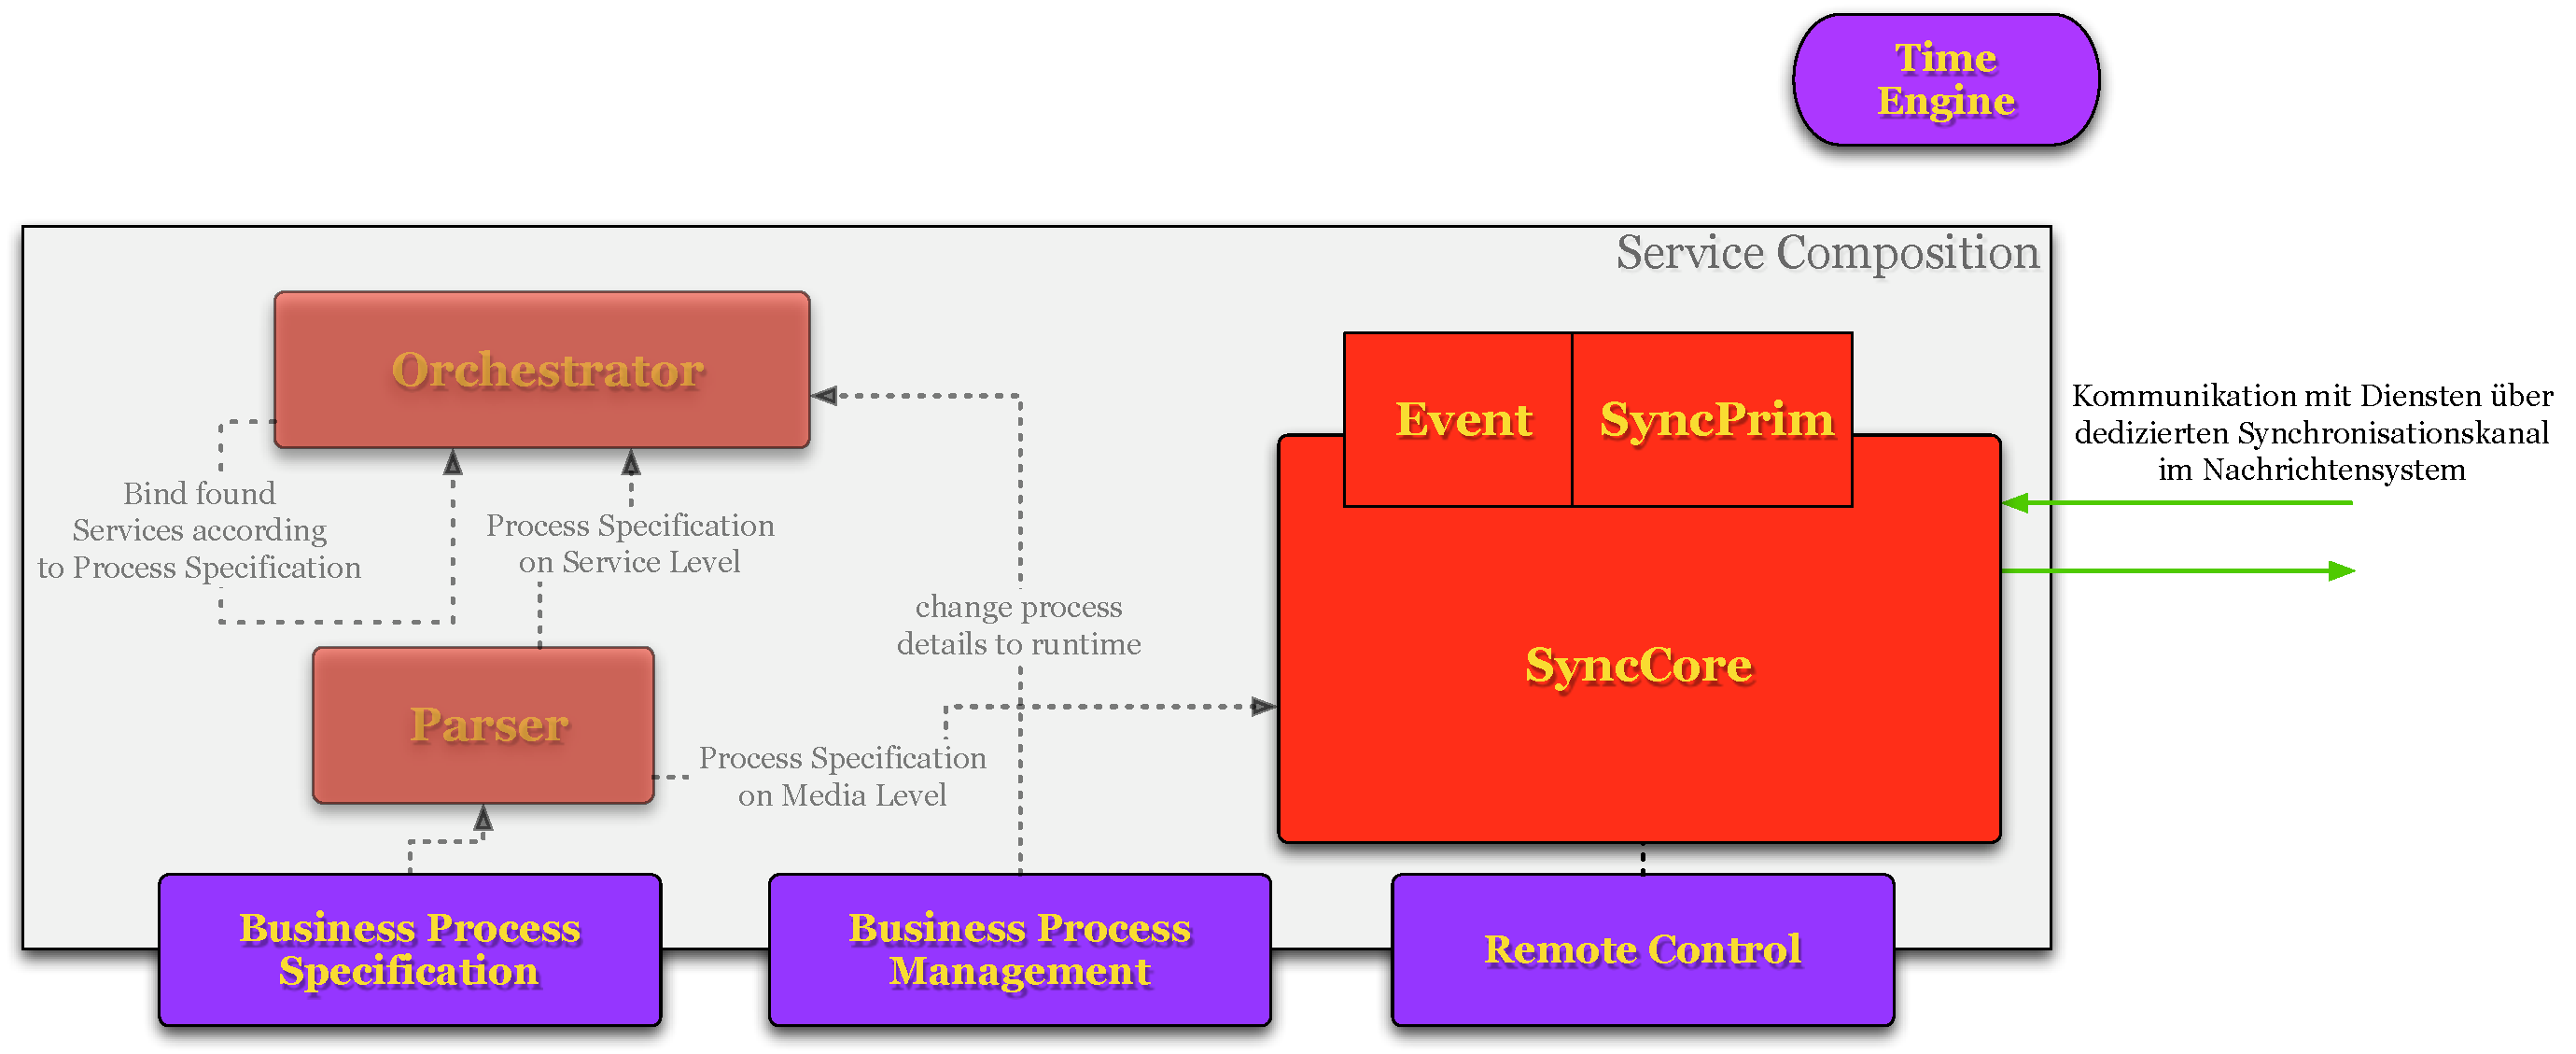
\includegraphics[width=.9\textwidth]{images/Servicekomposition_syncpart.pdf}
    \caption{Komponenten zur Synchronisation im COSIMA-Projekt}
    \label{fig:images_Servicekomposition_syncpart}
  \end{figure}
  
  In Abbildung \ref{fig:images_Servicekomposition_syncpart} sind noch einmal jene Komponenten in dem COSIMA-Projekt dargestellt, die die Funktionalitäten zur Synchronisation bereitstellen sollen. Sie lässen sich dabei jedoch nicht ohne weiteres auf eines der im vorherigen Abschnitt vorgestellten Referenzmodelle übertragen, da diese vor allem für lokale Umgebung konzeptioniert sind. Um eine Synchronisation in einer verteilten Umgebung, wie COSIMA zu realisieren, sind zusätzliche Mechanismen und Komponenten notwendig~\citep[S. 608ff]{multimedia_technologie}. 
  
\paragraph{Besonderheiten bei verteilten Umgebungen} % (fold)
\label{par:besonderheiten_bei_verteilten_umgebungen}

  Das Problem, dass es in verteilten Umgebungen zu lösen gilt, besteht darin, dass Medienobjekte und Synchronisationsinformationen an unterschiedlichen Stellen vorgehalten werden~\citep[S. 607]{multimedia_technologie}. Eine Möglichkeit dieses Problem zu lösen, ist die Etablierung eines separaten Kanals\footnote{Dieser Kanal ist in der erweitere SOA nach Papazoglou auf Ebene der komponierten Dienste einzuordnen (siehe auch \ref{ssub:definition_dienstorientierte_architektur}).}, über den die Synchronisationsinformationen übertragen werden können~\citep[S. 608]{multimedia_technologie}. Die Synchronisation unterschiedlicher Medienobjekte wird in diesem Fall von einer Consumer-Komponente übernommen~\citep[S. 608]{multimedia_technologie}. Eine Alternative dazu wäre die Synchronisation in der Producer (oder Transformer) Komponente. Dazu werden die zu synchronisierenden Medien in einem \emph{Multiplex}-Datenstrom zusammengefasst und erst anschließend übertragen.
  
  Des Weiteren ist es notwendig einen globalen Zeitgeber einzuführen, um eine zeitliche Koordination der unterschiedlichen Komponenten zu erreichen~\citep[S. 610]{multimedia_technologie}. Diese Aufgabe wird im COSIMA-Projekt von der \emph{Time-Engine} Komponente realisiert.

% paragraph besonderheiten_bei_verteilten_umgebungen (end)  

\paragraph{Spezifikation von Synchronisation} % (fold)
\label{par:spezifikation_von_synchronisation}

  Unabhängig dieser Besonderheiten, lässt sich das Synchronisationsmodell innerhalb von COSIMA am ehesten dem Referenzmodell von Meyer und Steinmetz zu ordnen. Dabei entsprich die Spezifikationsschicht in COSIMA der Komponente der Servicekomposition mit deren Subkomponente des \emph{SyncCore}. Die Spezifikation der Synchronisationsanforderungen kann grundsätzlich über unterschiedliche Modell erfolgen, Bertino und Ferrari haben diese in~\citep[S. 617]{bertino1998tsm} wie folgt zusammengefasst:
  
  \begin{itemize}
    \item Graphen-basierte Modelle, 
    \item Petri-Netz basierte Modelle, 
    \item Objektorientierte Modelle sowie 
    \item sprach-basierte Modelle.
  \end{itemize}
  
  Grundsätzlich wurde bereits in~\citep[S. 34]{bericht} darauf hingewiesen, dass unterschiedliche Modelle unterstützt werden müssen. Die Modellierung des Medienobjekt ($\to$ \ref{ssub:medienobjekt}) basiert konkret jedoch bereits auf einem Objektorientierten Modell. Zu diesem Zeitpunkt kann dadurch die Verwendung eines der anderen Modelle jedoch nicht ausgeschlossen werden.

  Die konkrete Ausführung dieser Spezifikation kann dabei auf zwei Arten geschehen. Zum einen Ereigniss-gesteuert, also nicht-deterministisch\footnote{Relevant etwa bei Benutzer-Interaktionen oder Ausnahmebehandlungen}, wie sie unter anderem bei~\citep{little1991ms} und~\citep{bertino1998tsm} beschrieben wird\footnote{Diese Sychronisationsbehandlung lässt sich sehr gut in COSIMA integrieren, da auch innerhalb einer dienstorientierten Architektur eine starke Ereignisorientierung anzustreben ist, um ein Maximum an Flexibilität zu erhalten~\citep[S. 96]{masak2007ssb}}. Zum anderen ist noch eine Synchronisation über sogenannte \emph{Synchronisationsprimitive}, wie sie unter anderem bei~\citep{gaggi2005msh} beschrieben wird, vorgesehen.
  
% paragraph spezifikation_von_synchronisation (end)

  Die Objektschicht entspricht innerhalb von COSIMA dem Medienobjekt ($\to$ \ref{ssub:medienobjekt}) und dem Media Broker ($\to$ \ref{ssub:media_broker}), die im nächsten Abschnitt eingehender beschrieben werden.
  
  Die Stromschicht und Medienschicht sind bisher nicht explizit in COSIMA modelliert und sollten auch vollständig über das Medienobjekt für die Architektur abstrahiert werden. Eine Auseinandersetzung mit diesen Schichten sollte ausschließlich innerhalb der medienverarbeitenden Komponenten ($\to$ \ref{sub:medienverarbeitende_komponenten}) geschehen. Dadurch kann die Multimediaanwendungen auch nicht länger direkt auf alle Schichten zugreifen, wie es noch in dem Referenzmodell vorgesehen war~\citep[S. 13]{blakowski1996mss}: Aus Sicht der Servicekomposition kann nur auf die Spezifikationsschicht zugegriffen werden. Aus Sicht der medienverarbeitenden Komponenten ist nur die Objektschicht sichtbar, die gekapselt die anderen Schichten bereitstellt.

  Die gesamte Thematik der Synchronisation ist sehr komplex und eine Vielzahl von Aspekten müssen betrachtet werden~\citep[S. 27ff]{bericht}. In dieser Arbeit soll das grundsätzliche Konzept der Architektur im COSIMA-Projekt validiert werden, daher wird im Rahmen des Szenarios eine sehr einfache Betrachtung dieser Thematik durchgeführt und später entsprechend implementiert. Wesentlich umfangreicher wird dieses Thema hingegen bei~\citep{antons09} behandelt. Dort wird eine nachrichtenbasierte Synchronisation im Zusammenhang von Streaming angestrebt, die auf Basis von \emph{Message Exchange Pattern} (MEP\abk{MEP}{Message Exchange Pattern}) realisiert werden soll. Auch der Frage, ob drei Granularitätsstufen bei der Betrachtung von Synchronisation von Vorteil sind, wird sich dort eingehender gestellt.

% minisec umsetzung_in_cosima (end)

% subsubsection synchronisation (end)
  
\subsubsection{Medienobjekt} % (fold)
\label{ssub:medienobjekt}

  Im Zusammenhang von Synchronisation findet sich in der Literatur immer wieder der Begriff des \emph{Medienobjekts}. Auch in dem Komponentenbasierten Multimediarahmenwerk MET++~\citep{ackermann1994dai} wird ein Medienobjekt modelliert. Folglich sollte auch im COSIMA-Projekt ein dediziertes Medienobjekt modelliert werden~\citep{bericht}. Ergebnis dieser Modellierung ist das \emph{Medienobjekt} und der \emph{Media Broker}, die in diesem Abschnitt näher beschrieben werden.

  Es wurde bereits in Abschnitt~\ref{ssub:nachrichtensystem} erläutert, dass in einer dienstorientierten Architektur der Datenfluss durch die Nachrichtenvermittlung realisiert wird\footnote{Obwohl der Kontrollfluss auch durch die Nachrichtenvermittlung realisiert werden kann, stehen in diesem Zusammenhang die Daten im Vordergrund.}. In den vorherigen Abschnitten wurde jedoch deutlich, dass Multimediadaten mitunter spezielle Anforderungen an ihre Vermittlung stellen. Um überhaupt eine Vermittlung von Medien zu realisieren, wie sie im nächsten Abschnitt beschrieben wird, muss jedoch zuvor eine Repräsentation von Medien entwickelt werden, die sich für den Einsatz in dienstorientierten Architekturen eignet. Vor diesem Hintergrund wurde das \emph{Medienobjekt} in COSIMA mit den folgenden Anforderungen modelliert~\citep[S. 34]{bericht}:
  
  \begin{description}
    \item[Erweiterbarkeit] Das COSIMA-Projekt soll Verwendung zur Entwicklung von Multimediaanwendungen in sehr vielen Domänen finden. Daher muss das Medienobjekt sich an diese Domänen leicht adaptieren lassen. Dies könnte durch eine abstrakte Darstellung der Eigenschaften von Medien erreicht werden.
    \item[Metadaten] Dort wo Medien verwendet werden, findet sich in den meisten Fällen auch eine Beschreibung dieser Medien. Diese Metadaten sind daher ebenso als \emph{first-class citizen} zu betrachten und inhärent im Medienobjekt verankert sein.
    \item[Streaming] Beim Umgang mit Medien, vor allem mit kontinuierlichen Medien spielen fast immer auch Datenströme, oder auch \emph{Streaming} eine wesentliche Rolle~\citep[S. 14ff]{multimedia_technologie}. Aus diesem Grund muss das Medienobjekt Streaming explizit vorsehen. Eng verbunden mit dem Streaming ist die \emph{Dienstgüte}~\citep{multimedia_technologie} und muss daher ebenfalls berücksichtigt werden.
    \item[Verteilung] In einer dienstorientierten und damit potentiell verteilten Architektur müssen auch die Medien verteilt zu prozessieren sein. Innerhalb des Medienobjektes müssen also dementsprechende Voraussetzungen geschaffen werden.
    \item[Synchronisation] Wie bereits in Abschnitt~\ref{ssub:synchronisation} erläutert, ist es für eine Multimediaarchitektur inhärent notwenig die Synchronisation der Medien abzubilden. Neben den bereits beschriebenen Komponenten muss auch das Medienobjekt entsprechend dieser Anforderung modelliert werden.
  \end{description}

  Das Klassendiagramm in Abbildung \ref{fig:medienobjekt} zeigt das Medienobjekte in COSIMA und seine relevanten assoziierten Klassen. Im weiteren Verlauf werden die wesentlichen Merkmale des Medienobjekts im Detail beschrieben.
  
  \begin{figure}[!ht]
    \centering
      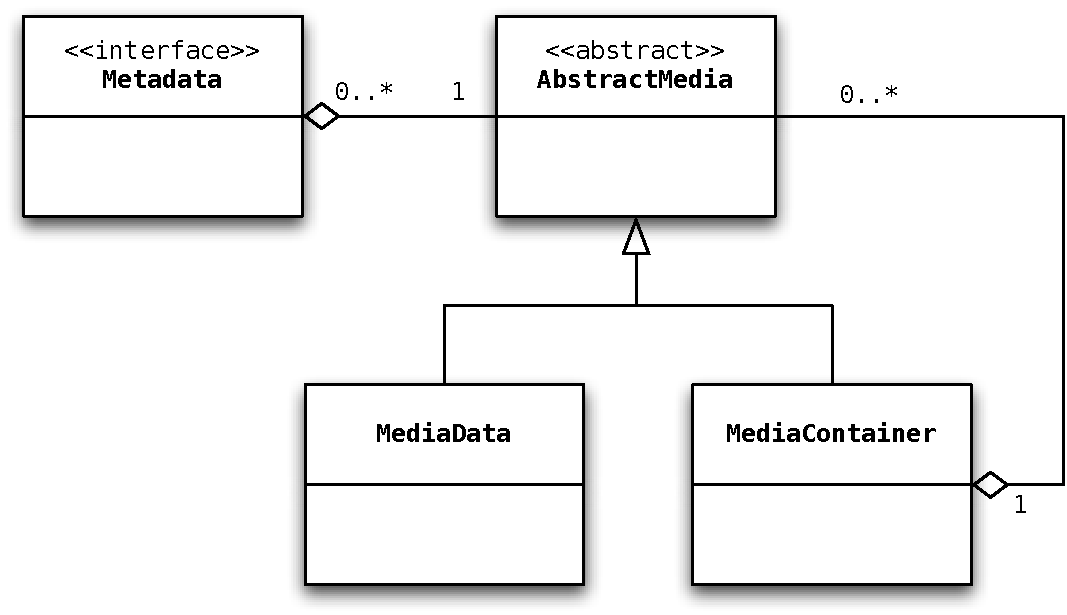
\includegraphics[width=.9\textwidth]{images/Medienobjekt.pdf}
    \caption{Klassendiagramm des Medienobjektes}
    \label{fig:medienobjekt}
  \end{figure}

\minisec{Eigenschaften des Medienobjektes} % (fold)
\label{msec:eigenschaften_des_medienobjektes}

  Ähnlich der LDUs, wie sie bei Meyer und Steinmetz beschrieben sind\footnote{siehe dazu auch Abschnitt \ref{msec:modelle_zur_beschreibung_zeitlicher_synchronisation}} kennt auch das Medienobjekt unterschiedliche Granularitätsstufen von Medien\footnote{Im Falle eines Videos wäre folgende Hierarchie denkbar: \emph{Video} $\Rightarrow$ \emph{Szene} $\Rightarrow$ \emph{Einstellung} $\Rightarrow$ \emph{Einzelbild}}. Diese Funktionalität ist dabei über das \emph{Composite}-Entwurfsmuster~\citep[S. 163]{design_patterns} realisiert.  Diese Hierarchie muss dabei jedoch in eine zeitliche Reihenfolge gebracht werden. Diese Aufgabe übernehmen dedizierte Synchronisationsobjekte, die selbst wieder als \emph{Composite} modelliert sind. Eine generelle Anordnung in der Zeitdomäne geschieht dabei über unterschiedliche \verb!EventGroup!-Instanzen. Die konkrete Umsetzung der Synchronisation übernehmen unterschiedliche \verb!TemporalWrapper!-Instanzen. Sie halten dabei Referenzen auf einzelne Medienobjekte (vgl. dazu auch~\citep[S. 84]{ackermann1996doo}).
  
  Diese Modellierung ist dabei stark an die Modellierung des MET++-Rahmenwerk angelehnt~\citep[S. 75]{ackermann1996doo}, im Gegensatz dazu werden medienspezifische Operationen wie \emph{Start}, \emph{Stop} oder \emph{Pause} in COSIMA nicht im Medienobjekt realisiert, sondern in den verantwortlichen Diensten\footnote{Dadurch werden die Medienobjekte wesentlich leichtgewichtiger und die Prozessierungslogik auf die Dienst ausgelagert.}.
  
  \abk{MPEG-7}{The Multimedia Content Description Interface}
  \abk{COMM}{Core Ontology for MultiMedia}
  
  Zur Integration von beliebigen Metadaten, kann die sehr einfache \verb!Metadata!-Schnittstelle implementiert werden. Obgleich auch als Metadaten zu interpretieren, wird die Möglichkeit zur Beschreibung des Inhalts der Medien (etwa durch MPEG-7\footnote{\url{http://www.chiariglione.org/mpeg/standards/mpeg-7/mpeg-7.htm}}) von einer separaten Komponente realisiert, der \verb!ContentDescriptor!-Klasse. Neben MPEG-7 sollte für COSIMA ebenfalls die Multimedia Ontolgie COMM~\citep{arndt2007cdw} zur Beschreibung von Inhalten in Betracht gezogen werden. Sie setzt auf MPEG-7 auf und bietet eine wesentlich bessere Integration in webbasierte Umgebungen als MPEG-7~\citep[S. 31]{arndt2007cdw}.
  
  Eine weitere wesentliche Eigenschaft des Medienobjekts ist, dass es selbst nicht die eigentlichen Mediendaten enthält, sondern lediglich in der Lage ist über die \verb!MediaStore!-Schnittstelle die extern gespeicherten Daten an die Anwendung durchzureichen. Jedes Medienobjekt lässt sich dafür über eine eindeutige URI\abk{URI}{Uniform Resource Identifier} in der Multimediaanwendungen referenzieren und sind somit lediglich reichhaltige Verweise auf die eigentlichen Daten. Die eigentlichen Daten liegen dabei in Form entsprechend geeigneter Formaten vor, damit ist die beschriebene Granularität der \emph{Composites} jeweils abhängig von der bereitgestellten Granularität des verwiesenen Datenformats.
  
  Bei einer Einordnung in das Referenzmodell von Meyer und Steinmetz, lässt sich erkennen, dass die Medienschicht nach Meyer und Steinmetz zwar zum Teil gekapselt wird, über die verschiedenen Composites Dienste jedoch Zugriff auf die jeweils kleinsten Einheiten erhalten. Des Weiteren ist die Stromschicht  in COSIMA nicht länger in der Applikation oder dem Rahmenwerk selbst realisiert, sondern wird durch externe Formate oder Protokolle bereitgestellt.
  
% minisec eigenschaften_des_medienobjekt (end)

  Wie diese Medienobjekte innerhalb einer Multimediaanwendungen vermittelt und übertragen werden sollen, stellt der folgende Abschnitt vor.

% subsubsection medienobjekt (end)

\subsubsection{Medien Broker} % (fold)
\label{ssub:media_broker}

  \begin{definition}[Broker]\label{def:broker}
    "`\textbf{1.} [engl. broker, eigtl. = Weinhändler]: Effektenhändler an der englischen und amerikanischen Börse."'\footnote{aus: Duden - Deutsches Universal Wörterbuch A-Z, 3. Aufl., 1996} "`\textbf{2.} One employed as a middleman to transact business or negotiate bargains between different merchants or individuals."'\footnote{aus: The Oxford English Dictionary, 3. Aufl., 1970} "`\textbf{3.} A middleman, intermediary, or agent generally; an interpreter, messanger, comissioner."'\footnote{aus: The Oxford English Dictionary, 3. Aufl., 1970}
  \end{definition}

  Als einen Broker kann man demnach einen Makler oder Vermittler zwischen zwei Parteien, die Informationen oder Waren austauschen wollen bezeichnen.

  Diese Bedeutung lässt sich auch im Umfeld von verteilten Systemen weitestgehend übernehmen\footnote{Hier ist beispielhaft der \emph{Object Request Broker} (ORB\abk{ORB}{Object Request Broker}) bei CORBA\abk{CORBA}{Common Object Request Broker Architecture} zu nennen~\citep{coulouris2001ds,balzert1999lo}.} und im Kontext der dienstorientierten Architekturen lässt sie sich auf den \emph{Message Broker} anwenden. Dieser stellt statt einer Punkt-zu-Punkt Verbindung zwischen Diensten, eine zentrale Vermittlungsstelle zur Verfügung~\citep[S. 71]{web_services}. Dabei muss es sich aber nicht immer um ein zentrales System handeln und wird in modernen Umgebungen zumeist als dezentrale Komponente realisiert~\citep{enterprise_service_bus}. Grundsätzlich kann auch gesagt werden, dass ein Broker dem \emph{Mediator} Pattern~\citep[S. 273]{design_patterns} in einer verteilten Umgebung entspricht~\citep[S. 83]{enterprise_integration_patterns}.
  
  Der Medien Broker bei COSIMA soll ähnliche Funktionen bei der Vermittlung von Medien zwischen den einzelnen Diensten übernehmen. Zur Zeit ist der Medien Broker so konzeptioniert, dass er die im vorherigen Abschnitt beschriebenen Medienobjekte zwischen den verschiedenen medienverarbeitenden Komponenten vermittelt. Obwohl er dadurch selbst auch nur Referenzen auf die eigentlichen Daten vermittelt, stellt er dennoch Adaptoren bereit, die einen konkreten Datenzugriff in einer verteilten Umgebung erlauben. Vorraussetzung dazu ist jedoch, die Verwendung eines Backends, dass eine verteilten Zugriff erlaubt. Ein sehr rudimentäres Backend würde ein NFS\abk{NFS}{Network File System} darstellen. Eine deutlich mächtigere Lösung stellt hingegen das \emph{MultiMonster}-Projekt\footnote{\url{http://www6.informatik.uni-erlangen.de/research/projects/retavic/multimonster/index.html}} dar. Dieser, von der Universität Erlangen entwickelte Multimediaserver kann Medien in einer Echtzeitumgebung bereitstellen und dabei unterschiedliche Dienstgüten gerecht werden. Zusätzlich ist er in der Lage Mediendaten in unterschiedliche Formate zu konvertieren, ist dabei plattformunabhängig und lässt sich leicht erweitern~\citep{suchomski2004oar}\footnote{Das M.e.T.t. Projekt hat sich bereits im Rahmen des COSIMA-Projekts prototypisch mit einer möglichen Integration beschäftigt: \url{https://mims01.gm.fh-koeln.de/twiki/bin/view/MIMaster/MeT}}.
  
  Der Medien Broker lässt sich in die erweiterte SOA nach Papazoglou (siehe Abbildung \ref{fig:images_Extended_SOA} auf Seite \pageref{fig:images_Extended_SOA}) als einen weiteren Kanal, neben dem Daten- und Kontrollkanal sowie Synchronisationskanal auf der Ebene der komponierten Dienste einordnen.
  
% subsubsection media_broker (end)

% section architektur (end)

\section{Offene Fragen} % (fold)
\label{sec:offene_fragen}

  In diesem Kapitel ist der Status Quo des COSIMA-Projekts vorgestellt worden. Die bereits in~\citep{bericht} konzipierte Architektur wurde im Rahmen dieser Arbeit, vor allem bei der Verwendung der Begriffe aus der SOA-Domäne, weiter gefestigt. Das hier vorgestellte soll des Weiteren als Grundlage für die prototypische Realisierung und szenariobasierte Validierung dienen.

  COSIMA ist ein junges Projekt und daher gilt es noch viele Punkte zu klären. Im Folgenden sollen die wichtigsten dieser Punkte kurz erläutert werden. Nur wenige der Fragen, die dadurch aufgeworfen werden, können in dieser Arbeit beantwortet werden. Abschließend kann wohl auf keine einzige eine hinreichende Antwort gefunden werden.
  
\subsection{Framework oder Architektur} % (fold)
\label{sub:framework_oder_architektur}

  In der Zieldefinition und dem Mission Statement des Projekts, wie sie zu Beginn dieses Kapitels und in~\citep{bericht} genannt wurden, wird noch von der Erstellung eines \emph{Frameworks} gesprochen. Scherp und Boll nennen in~\citep[S. 396f]{scherp2006fe} die folgenden drei Punkte als Eigenschaften von Frameworks:
  
  \begin{itemize}
    \item Umkehrung des Kontrollflusses
    \item Vorgabe einer konkreten Anwendungsarchitektur
    \item Anpassbarkeit durch Variationspunkte
  \end{itemize}
  
  Ohne im Detail auf diese Eigenschaften einzugehen, fällt jedoch schnell auf, dass der Punkt zur Umkehrung des Kontrollflusses sich nur schlecht mit den Konzepten einer dienstorientierten Architektur decken lässt: Der Servicekomposition liegt nach~\citep[S. 320]{web_services_principles_and_technology} ein \emph{Flow-Model} zu Grunde, dass, wie bereits in Abschnitt~\ref{sub:service_komposition} detailliert beschrieben, den Ablauf einer Applikation steuert. Und diese unterliegt dem direkten Einfluss des Anwendungsentwicklers, wie in Abbildung~\ref{fig:Kontextsicht_Architektur_COSIMA} deutlich zu erkennen ist. Aus Sicht des Anwendungsentwicklers handelt es sich demnach nicht um ein Rahmenwerk.
  
  Wird die Perspektive jedoch zu einem Dienstanbieter jedoch gewechselt, erfüllt COSIMA durchaus alle Kriterien, um als Rahmenwerk bezeichnet zu werden: Ihm wird eine konkrete Anwendungsarchitektur vorgegeben, er kann einige Eigenschaften gezielt beeinflussen und hat keinen Einfluss auf den Kontrollfluss.
  
  Diese Divergenz wird noch verstärkt, wenn die Spezifikation der Dienstkomposition, genauer betrachtet wird. Die Spezifikation wird lediglich deklarativ angegeben, ihre konkrete Ausführung selbst obliegt einer Komponente, auf die der Anwendungsentwickler nur wenig Einfluss nehmen kann. Ähnlich dem Optimieren von Anweisungen bei Compilern oder Datenbanken, kann auch in diesem Fall die eigentlich Ausführung deutlich anders aussehen, als sie von dem Anwendungsentwickler spezifiziert wurde. Demnach gibt tatsächlich auch der Anwendungsentwickler einen Teil des Kontrollflusses wieder an COSIMA ab.
  
  Es lässt sich demnach nicht eindeutig feststellen, ob es sich um ein Rahmenwerk oder eine reine Architektur handelt. Abhängig von der Sichtweise sind beide Charakterisierungen valide und können demnach so verwand werden. In weiteren Arbeiten muss dieser Januskopf jedoch weiterhin bedacht werden.

% subsection framework_oder_architektur (end)

\subsection{Servicekomposition} % (fold)
\label{sub:servicekomposition_fragen}

  Bei einer Weiterentwicklung muss in jedem Fall die Komponente der Servicekomposition weiter ausdifferenziert werden. Es muss eingehend die Eignung bestehender Sprachen zur Komposition von Diensten im Kontext von Multimediaanwendungen geprüft werden. Auch die Frage, ob eine Orchestrierung oder eine Choreographie vorzuziehen ist, oder eine Mischung aus beiden Ansätzen, wie sie auch bei~\citep{papazoglou2007soc} gefordert wird, muss geklärt werden.
  
  Ein weiterer Aspekt, der in den Verantwortungsbereich der Servicekomposition fällt, ist die Beachtung Nicht-Funktionalen Anforderungen einzelner Dienste~\citep[S. 42]{papazoglou2007soc}. Dieser Aspekt wurde bisher bewusst bei der Entwicklung des COSIMA-Projekts völlig ausgeblendet. Bei einer weiteren Entwicklung muss dieser Punkte daher unbedingt Berücksichtigung finden.

  Nach~\citep[S. 8]{service_oriented_computing} stehen im Kontext des \emph{Service-Oriented Computing} (SOC) komponierte Dienste für weitere Kompositionen zur Verfügung. Diese Möglichkeit ist zur Zeit nicht explizit in COSIMA modelliert worden. Auch für die Entwicklung von Multimediaanwendungen kann diese Fähigkeit von Vorteil sein. Welche Konsequenzen eine solche verschachtelte Komposition haben könnte, kann hier nicht abschließend geklärt werden und sollte daher Teil weiterer Forschung sein.
  
  Ebenfalls sollte evaluiert werden, inwiefern sich die Ergebnisse aus~\citep{samma08} in Bezug auf die Verwendung von BPEL\abk{BPEL}{Business Process Execution Language} und der dort vorgestellten Erweiterung von BPEL, \emph{BPEL for Multimedia} (BPEL-MM) in die jetzige Dienstkomposition integrieren lassen.

% subsection servicekomposition (end)

\subsection{Synchronisation} % (fold)
\label{sub:synchronisation}

  Es wurde gezeigt, dass Synchronisation ein elementares Element für jede Multimediaanwendung darstellt. Die Tiefe in der dieses Thema im Rahmen der vorliegenden Arbeit behandelt werden konnte, wird jener Relevanz jedoch nicht vollständig gerecht. So bleibt unter anderem die Frage offen, wie die Realisierung von Echtzeit-Anforderungen aussehen kann. Bei Steinmetz ist die Stromschicht in eine Echtzeitumgebung eingebettet~\citep[S. 604]{multimedia_technologie}, die Schichten darüber jedoch nicht mehr. In der jetzigen Modellierung wird die Stromschicht von einer externen Komponente realisiert. Bei Verwendung des MultiMonster-Medienservers ist dieser zwar echtzeitfähig eine echte Überprüfung für die Realisierung von Echtzeitanforderungen steht aber noch aus.
  
  Bei~\citep{antons09} wird eine Realisierung von Synchronisation über die Verwendung von Message Exchange Pattern und einem separaten Synchronisationskanal angestrebt. Ob dieser Ansatz zu einem optimalen Ergebnis führt, bleibt abzuwarten. In jedem Fall sollten andere Möglichkeiten evaluiert werden, verteilte Synchronisation umzusetzen.

% subsection synchronisation (end)

\subsection{ESB} % (fold)
\label{sub:esb_fragen}

  Bei der Realisierung eines Enterprise Service Bus muss die fundamentale Entscheidung getroffen werden, ob er API-getriebene oder Protokoll-getrieben implementiert werden soll~\citep[S. 59]{soa_in_practice}. Ohne diese beiden Ansätze an dieser Stelle weiter zu vertiefen, muss die Weiterentwicklung des Projekts sich für einen der beiden entscheiden.
  
  Es existieren eine Vielzahl von kommerziellen und nicht-kommerziellen ESB Lösungen. Deren Eignung für die Verwendung innerhalb des COSIMA-Projekts muss im Einzelnen geprüft werden. Bei dieser Integration ist jedoch zu beachten, dass COSIMA selbst bereits als ESB charakterisiert werden kann. Viele der genannten Eigenschaften lassen sich in der Architektur von COSIMA wieder finden. Es könnten demnach entweder Teile eines bestehenden ESB in COSIMA integriert werden, oder ein bestehender ESB um die Multimedia Charakteristika von COSIMA erweitert werden.

% subsection esb_fragen (end)

% section offene_fragen (end)

% chapter eine_dienstorientierten_multimediaarchitektur (end)
